% ******************************* PhD Thesis Template **************************
% Please have a look at the README.md file for info on how to use the template
%!TEX encoding = UTF-8 Unicode
\documentclass[a4paper,12pt,customfont,custombib,custommargin,index]{Classes/PhDThesisPSnPDF}
%\documentclass[a4paper,12pt,customfont,custombib,custommargin,print,index]{Classes/PhDThesisPSnPDF}

% ******************************************************************************
% ******************************* Class Options ********************************
% *********************** See README for more details **************************
% ******************************************************************************

% `a4paper'(The University of Cambridge PhD thesis guidelines recommends a page
% size a4 - default option) or `a5paper': A5 Paper size is also allowed as per
% the Cambridge University Engineering Deparment guidelines for PhD thesis
%
% `11pt' or `12pt'(default): Font Size 10pt is NOT recommended by the University
% guidelines
%
% `oneside' or `twoside'(default): Printing double side (twoside) or single
% side.
%
% `print': Use `print' for print version with appropriate margins and page
% layout. Leaving the options field blank will activate Online version.
%
% `index': For index at the end of the thesis
%
% `draftclassic': For draft mode without loading any images (same as draft in book)
%
% `draft': Special draft mode with line numbers, images, and water mark with
% timestamp and custom text. Position of the text can also be modified.
%
% `abstract': To generate only the title page and abstract page with
% dissertation title and name, to submit to the Student Registry
%
% `chapter`: This option enables only the specified chapter and it's references
%  Useful for review and corrections.
%
% ************************* Custom Page Margins ********************************
%
% `custommargin`: Use `custommargin' in options to activate custom page margins,
% which can be defined in the preamble.tex. Custom margin will override
% print/online margin setup.
%
% *********************** Choosing the Fonts in Class Options ******************
%
% `times' : Times font with math support. (The Cambridge University guidelines
% recommend using times)
%
% `fourier': Utopia Font with Fourier Math font (Font has to be installed)
%            It's a free font.
%
% `customfont': Use `customfont' option in the document class and load the
% package in the preamble.tex
%
% default or leave empty: `Latin Modern' font will be loaded.
%
% ********************** Choosing the Bibliography style ***********************
%
% `authoryear': For author-year citation eg., Krishna (2013)
%
% `numbered': (Default Option) For numbered and sorted citation e.g., [1,5,2]
%
% `custombib': Define your own bibliography style in the `preamble.tex' file.
%              `\RequirePackage[square, sort, numbers, authoryear]{natbib}'.
%              This can be also used to load biblatex instead of natbib
%              (See Preamble)
%
% **************************** Choosing the Page Style *************************
%
% `default (leave empty)': For Page Numbers in Header (Left Even, Right Odd) and
% Chapter Name in Header (Right Even) and Section Name (Left Odd). Blank Footer.
%
% `PageStyleI': Chapter Name next & Page Number on Even Side (Left Even).
% Section Name & Page Number in Header on Odd Side (Right Odd). Footer is empty.
%
% `PageStyleII': Chapter Name on Even Side (Left Even) in Header. Section Number
% and Section Name in Header on Odd Side (Right Odd). Page numbering in footer

% Uncomment to change page style
%\pagestyle{PageStyleII}

% ********************************** Preamble **********************************
% Preamble: Contains packages and user-defined commands and settings
% ******************************************************************************
% ****************************** Custom Margin *********************************

% Add `custommargin' in the document class options to use this section
% Set {innerside margin / outerside margin / topmargin / bottom margin}  and
% other page dimensions
\ifsetCustomMargin
  \RequirePackage[left=37mm,right=30mm,top=35mm,bottom=30mm]{geometry}
  \setFancyHdr % To apply fancy header after geometry package is loaded
\fi

% Add spaces between paragraphs
%\setlength{\parskip}{0.5em}
% Ragged bottom avoids extra whitespaces between paragraphs
\raggedbottom
% To remove the excess top spacing for enumeration, list and description
%\usepackage{enumitem}
%\setlist[enumerate,itemize,description]{topsep=0em}

% *****************************************************************************
% ******************* Fonts (like different typewriter fonts etc.)*************

% Add `customfont' in the document class option to use this section

\ifsetCustomFont
  % Set your custom font here and use `customfont' in options. Leave empty to
  % load computer modern font (default LaTeX font).
  %\RequirePackage{helvet}
%\usepackage{pxfonts}
\usepackage{amsfonts}
  % For use with XeLaTeX
  %  \setmainfont[
  %    Path              = ./libertine/opentype/,
  %    Extension         = .otf,
  %    UprightFont = LinLibertine_R,
  %    BoldFont = LinLibertine_RZ, % Linux Libertine O Regular Semibold
  %    ItalicFont = LinLibertine_RI,
  %    BoldItalicFont = LinLibertine_RZI, % Linux Libertine O Regular Semibold Italic
  %  ]
  %  {libertine}
  %  % load font from system font
  %  \newfontfamily\libertinesystemfont{Linux Libertine O}
\fi

% *****************************************************************************
% **************************** Custom Packages ********************************

% ************************* Algorithms and Pseudocode **************************

%\usepackage{algpseudocode}


% ********************Captions and Hyperreferencing / URL **********************

% Captions: This makes captions of figures use a boldfaced small font.
%\RequirePackage[small,bf]{caption}

\RequirePackage[labelsep=space,tableposition=top]{caption}
\renewcommand{\figurename}{Fig.} %to support older versions of captions.sty


% *************************** Graphics and figures *****************************

%\usepackage{rotating}
%\usepackage{wrapfig}

% Uncomment the following two lines to force Latex to place the figure.
% Use [H] when including graphics. Note 'H' instead of 'h'
%\usepackage{float}
%\restylefloat{figure}

% Subcaption package is also available in the sty folder you can use that by
% uncommenting the following line
% This is for people stuck with older versions of texlive
%\usepackage{sty/caption/subcaption}
\usepackage{subcaption}

% ********************************** Tables ************************************
\usepackage{booktabs} % For professional looking tables
\usepackage{multirow}

%\usepackage{multicol}
%\usepackage{longtable}
%\usepackage{tabularx}


% *********************************** SI Units *********************************
\usepackage{siunitx} % use this package module for SI units


% ******************************* Line Spacing *********************************

% Choose linespacing as appropriate. Default is one-half line spacing as per the
% University guidelines

% \doublespacing
% \onehalfspacing
% \singlespacing


% ************************ Formatting / Footnote *******************************

% Don't break enumeration (etc.) across pages in an ugly manner (default 10000)
%\clubpenalty=500
%\widowpenalty=500

%\usepackage[perpage]{footmisc} %Range of footnote options


% *****************************************************************************
% *************************** Bibliography  and References ********************

\usepackage{cleveref} %Referencing without need to explicitly state fig /table

% Add `custombib' in the document class option to use this section
\ifuseCustomBib
   %\RequirePackage[square, sort, numbers, authoryear]{natbib} % CustomBib

% If you would like to use biblatex for your reference management, as opposed to the default `natbibpackage` pass the option `custombib` in the document class. Comment out the previous line to make sure you don't load the natbib package. Uncomment the following lines and specify the location of references.bib file

%\RequirePackage[backend=biber, style=numeric-comp, citestyle=numeric, sorting=nty, natbib=true]{biblatex}
\RequirePackage[backend=biber, style=numeric-comp, sorting=nty, natbib=true]{biblatex}
\bibliography{References/references} %Location of references.bib only for biblatex

\fi

% changes the default name `Bibliography` -> `References'
\renewcommand{\bibname}{References}


% ******************************************************************************
% ************************* User Defined Commands ******************************
% ******************************************************************************

% *********** To change the name of Table of Contents / LOF and LOT ************

%\renewcommand{\contentsname}{My Table of Contents}
%\renewcommand{\listfigurename}{My List of Figures}
%\renewcommand{\listtablename}{My List of Tables}


% ********************** TOC depth and numbering depth *************************

\setcounter{secnumdepth}{2}
\setcounter{tocdepth}{2}


% ******************************* Nomenclature *********************************

% To change the name of the Nomenclature section, uncomment the following line

%\renewcommand{\nomname}{Symbols}


% ********************************* Appendix ***********************************

% The default value of both \appendixtocname and \appendixpagename is `Appendices'. These names can all be changed via:

%\renewcommand{\appendixtocname}{List of appendices}
%\renewcommand{\appendixname}{Appndx}

% *********************** Configure Draft Mode **********************************

% Uncomment to disable figures in `draft'
%\setkeys{Gin}{draft=true}  % set draft to false to enable figures in `draft'

% These options are active only during the draft mode
% Default text is "Draft"
%\SetDraftText{DRAFT}

% Default Watermark location is top. Location (top/bottom)
%\SetDraftWMPosition{bottom}

% Draft Version - default is v1.0
%\SetDraftVersion{v1.1}

% Draft Text grayscale value (should be between 0-black and 1-white)
% Default value is 0.75
%\SetDraftGrayScale{0.8}


% ******************************** Todo Notes **********************************
%% Uncomment the following lines to have todonotes.

%\ifsetDraft
%	\usepackage[colorinlistoftodos]{todonotes}
%	\newcommand{\mynote}[1]{\todo[author=kks32,size=\small,inline,color=green!40]{#1}}
%\else
%	\newcommand{\mynote}[1]{}
%	\newcommand{\listoftodos}{}
%\fi

% Example todo: \mynote{Hey! I have a note}

% using japanese charater package
\usepackage{CJKutf8}

\usepackage{setspace}


% ************************ Thesis Information & Meta-data **********************
% Thesis title and author information, refernce file for biblatex
% ************************ Thesis Information & Meta-data **********************
%% The title of the thesis
%!TEX encoding = UTF-8 Unicode
\title{New Approach of Numerical Relativity}
\titlechinese{數值廣義相對論的新方法}
%\texorpdfstring is used for PDF metadata. Usage:
%\texorpdfstring{LaTeX_Version}{PDF Version (non-latex)} eg.,
%\texorpdfstring{$sigma$}{sigma}

%% Subtitle (Optional)
\subtitle{Implementation, tests and applications}
\subtitlechinese{實施、測試和應用}

%% The full name of the author
\author{LAM, Tsz-lok}
\authorchinese{林子樂}

%% Department (eg. Department of Engineering, Maths, Physics)
%\dept{Department of Physics}

%% University and Crest
\university{The Chinese University of Hong Kong}

% Crest minimum should be 30mm.
%\crest{
\includegraphics[width=0.5\textwidth]{Figs/CUHK.png}}
%% Use this crest, if you are using the college crest
%% Crest long miminum should be 65mm
%\crest{\includegraphics[width=0.45\textwidth]{University_Crest_Long}}

%% College shield [optional] 
% Crest minimum should be 30mm.
%\collegeshield{\includegraphics[width=0.2\textwidth]{CollegeShields/Kings}}


%% Supervisor (optional)
%% for multiple supervisors, append each supervisor with the \newline command
\supervisor{Prof. Tjonnie G.F. LI}
%Prof. C.D. Supervisor}

%% Supervisor Role (optional) - Supervisor (default) or advisor
% \supervisorrole{\large\textbf{Supervisor: }}
%% if no title is desired:
%\supervisorrole{}

%% Supervisor line width: required to align supervisors
%\supervisorlinewidth{0.35\textwidth}

%% Advisor (optional)
%% for multiple advisors, append each advisor with the \newline command
%\advisor{{Dr. George Harrison\newline
%Dr. Ringo Starr}}
     
%% Advisor Role (optional) - Advisor (default) or leave empty
% \advisorrole{\normalsize\textbf{Advisors: }}
%% if no title is required
% \advisorrole{}

%% Advisor line width: required to align supervisors
%\advisorlinewidth{0.35\textwidth}


%% You can redefine the submission text:
% Default as per the University guidelines:
% ``This dissertation is submitted for the degree of''
\renewcommand{\submissiontext}{A Thesis Submitted in Partial Fulfilment \\ of the Reqirements for the Degree of}

%% Full title of the Degree
\degreetitle{Master of Philosophy \\ in \\ Physics}

%% College affiliation (optional)
%\college{Graduate School of Science}

%% Submission date
% Default is set as {\monthname[\the\month]\space\the\year}
\degreedate{July 2021} 

%% Meta information
\subject{LaTeX} \keywords{{LaTeX} {MPhil Thesis} {Physics} {The Chinese University of Hong Kong}}


% ***************************** Abstract Separate ******************************
% To printout only the titlepage and the abstract with the PhD title and the
% author name for submission to the Student Registry, use the `abstract' option in
% the document class.

\ifdefineAbstract
 \pagestyle{empty}
 \includeonly{Declaration/declaration, Abstract/abstract}
\fi

% ***************************** Chapter Mode ***********************************
% The chapter mode allows user to only print particular chapters with references
% Title, Contents, Frontmatter are disabled by default
% Useful option to review a particular chapter or to send it to supervisior.
% To use choose `chapter' option in the document class

%\ifdefineChapter
% \includeonly{Chapter3/chapter3}
%\fi

% ******************************** Front Matter ********************************
\begin{document}
\begin{CJK}{UTF8}{ipxm}

\frontmatter

\maketitle

%% ******************************* Thesis Dedidcation ********************************

\begin{dedication} 

I would like to dedicate this thesis to my loving parents \dots

\end{dedication}
%% ******************************* Thesis Declaration ***************************

\begin{declaration}

I hereby declare that except where specific reference is made to the work of 
others, the contents of this dissertation are original and have not been 
submitted in whole or in part for consideration for any other degree or 
qualification in this, or any other university. This dissertation is my own 
work and contains nothing which is the outcome of work done in collaboration 
with others, except as specified in the text and Acknowledgements. This 
dissertation contains fewer than 65,000 words including appendices, 
bibliography, footnotes, tables and equations and has fewer than 150 figures.

% Author and date will be inserted automatically from thesis.tex \author \degreedate

\end{declaration}
%% ************************** Thesis Acknowledgements **************************

\begin{acknowledgements}      


And I would like to acknowledge ...


\end{acknowledgements}

% ******************************* Thesis Committee ***************************

\begin{committee}
\vspace{0.9cm}
    \Large
	\textrm{Professor \textsc{Chu} Ming Chung (Chair)}

\vspace{0.4cm}

    \textrm{Professor \textsc{Li} Tjonnie Guang Feng (Thesis Supervisor)}

\vspace{0.4cm}

	\textrm{Professor \textsc{Ng} Kenny Chun Yu (Committee Member)}

\vspace{0.4cm}

    \textrm{Professor \textsc{Font} José Antonio (External Examiner)}

\end{committee}

% ************************** Thesis Abstract *****************************
% Use `abstract' as an option in the document class to print only the titlepage and the abstract.
\begin{abstract}
This is where you write your abstract ...
\end{abstract}

% ************************** Thesis Abstract *****************************
% Use `abstract' as an option in the document class to print only the titlepage and the abstract.
\begin{abstract_chinese}
\begin{CJK*}{UTF8}{bsmi}
{\CJKfamily{bkai}
許多天體物理場景都涉及中子星和黑洞,
例如核心坍縮超新星、雙中子星和中子星-黑洞合併,
它們是引力波物理學和多信使天體物理學中最重要的事件。
為了在合理的時間和負擔得起的計算資源內準確地對這些系統進行數值模擬,
需要多尺度、多維、完全並行、支持不同幾何形狀的通用相對論(磁)流體動力學代碼。
我們開發了新的開源、並行化、塊網格自適應、多維廣義相對論電磁流體動力學代碼 \underline{豬緲妞}(廣義相對論多重網格數值求解器),
用於動態時空曲線幾何。\\
\underline{豬緲妞} 碼流採用共形平坦度條件近似,
通過多重網格方法求解橢圓度量方程。
儘管 \underline{豬緲妞} 代碼在基準測試和苛刻的磁流體動力學問題中表現出色,
但保形平坦度條件近似阻止了模擬中引力波的發射。
具有完全廣義相對論處理的數值模擬能夠模擬從各種天體物理事件發出的引力波信號,
例如緻密二元聚結和核心坍縮超新星。
因此,
有必要擴展我們的代碼以採用完全約束公式,
這是從保角平坦度條件近似自然推廣的完全廣義相對論公式。
與廣義相對論的全雙曲公式相比,
全約束公式通過選擇最大切片條件和廣義狄拉克規範,
在每個時間步中最大化橢圓方程的數量,
雙曲扇區只留下兩個自由度這對應於遠場區域的引力波。
使用多重網格求解器,
橢圓度量方程可以在笛卡爾、圓柱或球面幾何中進行多維求解。\\
我們介紹了 \underline{豬緲妞} 中完全約束公式的方法、實現細節和性能。}
\end{CJK*}
\end{abstract_chinese}

% ******************************* Thesis Committee ***************************

\begin{conventions}
Unless explicitly stated, we adopt the geometrized Heaviside-Lorentz units,
for which the speed of light $c$, gravitational constant $G$, solar mass $M_\odot$,
vacuum permittivity $\epsilon_0$ and vacuum permeability $\mu_0$ are all equal to one
$(c=G=M_\odot =\epsilon_0 =\mu_0 =1)$.
Greek indices (e.g. $\mu, \nu, \rho, \sigma, \dots$), 
running from 0 to 3,
are used for 4-quantities 
while the Roman indices (e.g. $i,j,k,\dots$), 
running from 1 to 3, are used for 3-quantities.

\end{conventions}


% *********************** Adding TOC and List of Figures ***********************

\tableofcontents

\listoffigures

\listoftables

% \printnomenclature[space] space can be set as 2em between symbol and description
%\printnomenclature[3em]

\printnomenclature

% ******************************** Main Matter *********************************
\mainmatter

% ******************************* Part I ***************************************
\part{Methodology: Formulations}\label{part1}
%!TEX root = ../thesis.tex
%*******************************************************************************
%*********************************** First Chapter *****************************
%*******************************************************************************

\chapter{Introduction}  %Title of the First Chapter

\ifpdf
    \graphicspath{{Chapter1/Figs/PDF/}{Chapter1/Figs/}}
\else
    \graphicspath{{Chapter1/Figs/}}
\fi


%********************************** %First Section  **************************************
\section{Introduction to General Relativity} %Section - 1.1 
\label{section1.1}

\subsection{Einstein Field Equation} %Section - 1.1.1
\label{section1.1.1}

\begin{align} \label{eq:Einstein_eq}
    G_{\mu\nu} = 8 \pi T_{\mu\nu}
\end{align}

\subsection{Relativistic Star} %Section - 1.1.2
\label{section1.1.2}

\subsection{Gravitational Wave} %Section - 1.1.3
\label{section1.1.3}

%********************************** %Second Section  *************************************
\section{\texttt{Gmunu}: A general-relativistic electro-magneto-hydrodynamics code for generic astrophysical simulations} %Section - 1.2

%********************************** % Third Section  *************************************
\section{Outline of this thesis}  %Section - 1.3 
\label{section1.3}

%********************************** % Forth Section  *************************************
\section{Units and Convention}  %Section - 1.4
\label{section1.4}


%!TEX root = ../thesis.tex
%*******************************************************************************
%*********************************** Second Chapter *****************************
%*******************************************************************************

\chapter{Formulations of Einstein Field Equations}  %Title of the Second Chapter

\ifpdf
    \graphicspath{{Chapter2/Figs/PDF/}{Chapter2/Figs/}}
\else
    \graphicspath{{Chapter2/Figs/}}
\fi


%********************************** %First Section  **************************************
\section{Introduction} %Section - 2.1
\label{section2.1}

Due to the complexity and nonlinearity of Einstein field equations, it is extremely difficult to obtain analytical solution even for the simplest dynamical evolution systems.
Therefore, the accurate discription of the such systems can only be derived through numerical simulation.
For this, we need to reformulate the Einstein equations as an initial-value problem or Cauchy problem.
In this chapter, we will introduction the Arnowitt-Deser-Misner (ADM) formulation, which is the foundation of the 3+1 numerical relativity.
In particular, we will focus on the constrained scheme for the Einstein equations.

%********************************** %Second Section  *************************************
\section{The 3+1 decomposition of spacetime} %Section - 2.2 
\label{section2.2}
\subsection{Foliation of spacetime} \label{section2.2.1}

In the 3+1 decomposition, the spacetime manifold $\mathcal{M}$ is foliated into a set of non-intersecting spacelike hypersurfaces $\Sigma_t$ parameterized by the coordinate time $t$ \cite{misner1973gravitation}.
We denote a future-directed timelike unit four-vector $n^\mu$ normal to the hypersurface $\Sigma_t$ (i.e. $n_{\mu} \propto \nabla_\mu t$).
The induced spacetime metric $\gamma_{\mu\nu}$ on each hypersurfuce can then be defined as
\begin{align}\label{eq:2.2.spatial}
    \gamma_{\mu\nu} \coloneqq g_{\mu\nu} + n_{\mu} n_{\nu}.
\end{align}
Thus, we can construct spatial projection tensor $\gamma^{\mu}{}_{\nu}$ and time projection tensor $N^{\mu}{}_{\nu}$ as
\begin{align}
    \gamma^{\mu}{}_{\nu} &\coloneqq \delta^{\mu}{}_{\nu} + n^{\mu} n_{\nu}, & N^{\mu}{}_{\nu} &\coloneqq - n^{\mu} n_{\nu},
\end{align}
which decompose any generic four-vector $U^\mu$ into spatial part $\gamma^{\mu}{}_{\nu}U^{\nu}$ and timelike part $N^{\mu}{}_{\nu}U^{\nu}$.
Therefore, we can decompose the timelike vector field
\begin{align}\label{eq:2.2.1.normal_decompose}
t^\mu = \alpha n^{\mu} + \beta^{\mu}
\end{align}
into two components as
\begin{align}
    \alpha &\coloneqq - t^\mu n_\mu, & \beta^{\mu} &\coloneqq t^{\nu} \gamma^{\mu}{}_{\nu},
\end{align}
where the lapse function $\alpha$ measures the physical proper time ($\alpha\Delta t$) between two neighboring spatial hypersurface $\Sigma_t$ and $\Sigma_{t+\Delta t}$
, and the shift vector $\beta^i$ measures the changes of spatial coordinates on $\Sigma_{t+\Delta t}$.\\
Here, we summarise several useful relations.
The timelike normal vector $n^\mu$ and its corresponding one-form $n_\mu$ can be expressed as
\begin{align} \label{eq:2.2.1.normal}
    n^\mu &= \frac{1}{\alpha}\left(1, \beta^i \right), & n_\mu &= \left(\alpha, \vec{0}, \right).
\end{align}
The generic line element in 3+1 decomposition is given by
\begin{align}
    ds^2 = - \left( \alpha^2 - \beta^i \beta_i \right) dt^2 + \beta_i dx^i dt + \gamma_{ij} dx^i dx^j
\end{align}
The covariant and contravariant components of the metric can be written as
\begin{align}\label{eq:2.2.1.g}
    g_{\mu\nu} &= 
    \begin{pmatrix}
        - \alpha^2 + \beta^i \beta_i & \beta_j \\
        \beta_i & \gamma_{ij}
    \end{pmatrix}, &
    g^{\mu\nu} &= 
    \begin{pmatrix}
        - \frac{1}{\alpha^2} & \beta^j \\
        \beta^i & \gamma^{ij}
    \end{pmatrix}.
\end{align}
From equation(\ref{eq:2.2.1.g}), we can conclude that
\begin{align}
    \sqrt{-g} = \alpha \sqrt{\gamma},
\end{align}
where $g \coloneqq \det{\left(g_{\mu\nu}\right)}$ and $\gamma \coloneqq \det{\left(\gamma_{ij}\right)}$.

\subsection{Derivative operator} \label{section2.2.2}
With the 3+1 decomposition, we can now construct the 3-dimensional covariant derivative $D_\alpha$ associated with $\gamma_{\mu\nu}$ by projecting the 4-dimensional covariant derivative $\nabla_\alpha$ onto $\Sigma_t$, which is given by
\begin{align}\label{eq:2.2.2.spatialD}
    D_{\alpha} T^{\mu_1 \mu_2 \dots}{}_{\nu_1 \nu_2 \dots} = \gamma_{\alpha}{}^{\beta}\gamma_{\rho_1}{}^{\mu_1} \gamma_{\rho_2}{}^{\mu_2} \dots \gamma_{\nu_1}{}^{\sigma_1} \gamma_{\nu_2}{}^{\sigma_2} \dots \nabla_{\beta} T^{\rho_1 \rho_2 \dots}{}_{\sigma_1 \sigma_2 \dots},
\end{align}
for arbitrary tensor $T^{\mu_1 \mu_2 \dots}{}_{\nu_1 \nu_2 \dots}$ on spatial hypersurface $\Sigma_t$.
Using equation(\ref{eq:2.2.2.spatialD}), it can be shown that the corvariant derivative of $\gamma_{\mu\nu}$ vanishes
\begin{align}
\begin{split}
    D_{\alpha} \gamma_{\mu\nu} &= \gamma_{\alpha}{}^{\beta} \gamma_{\rho}{}^{\mu} \gamma_{\nu}{}^{\sigma} \nabla_{\beta} \left(g_{\rho\sigma} + n_\rho n_\sigma \right) \\
    &= \gamma_{\alpha}{}^{\beta} \gamma_{\rho}{}^{\mu} \gamma_{\nu}{}^{\sigma} \left( n_\rho \nabla_\beta n_\sigma + n_\sigma \nabla_\beta n_\rho \right) = 0
\end{split}
\end{align}
The components of 3-dimensional connection coefficients $\Gamma^{\alpha}{}_{\mu\nu}$ in coordinate basis can be expressed as
\begin{align}\label{eq:3_connection}
    \Gamma^{\alpha}{}_{\mu\nu} &= \frac{1}{2} \gamma^{\alpha\beta} \left( \partial_{\nu}\gamma_{\beta\mu} + \partial_{\mu}\gamma_{\beta\nu} - \partial_{\beta}\gamma_{\mu\nu} \right).
\end{align}
Here, the upper left index ${}^{(4)}$ marks the 4-dimensional tensors while the unmarked one represents purely spatial 3-dimensional tensors.
Similarly, the 3-dimensional Riemann tensor $R^{\alpha}{}_{\beta\mu\nu}$ associated with $\gamma_{\mu\nu}$ is defined by requiring that
\begin{align}
    2 D_{[\nu} D_{\mu]} W_\beta &= W_\alpha R^\alpha{}_{\beta\mu\nu}, & R^{\alpha}{}_{\beta\mu\nu} n_\alpha &= 0,
\end{align}
which can be explicitly expressed in coordinate basis as
\begin{align}
    R^{\alpha}{}_{\beta\mu\nu} &= \partial_{\mu} \Gamma^{\alpha}{}_{\beta\nu} - \partial_{\nu} \Gamma^{\alpha}{}_{\beta\mu} + \Gamma^{\alpha}{}_{\mu\rho}\Gamma^{\rho}{}_{\beta\nu} - \Gamma^{\alpha}{}_{\nu\rho}\Gamma^{\rho}{}_{\beta\mu}.
\end{align}
The 3-dimensional Ricci tensor $R_{\mu\nu}$ and Ricci scalar $R$ are defined in a similar manner as their 4-dimensional counterparts
\begin{align}
     R_{\mu\nu} &\coloneqq  R^\alpha{}_{\mu\alpha\nu}, & R &\coloneqq  R^{\mu}{}_{\mu}.
\end{align}
Since $R^{\alpha}{}_{\beta\mu\nu}$ is purely spatial and can be computed by the spatial derivatives of the spatial metric alone,
it only contains about information about the curvature intrinsic to the hypersurface $\Sigma_t$,
but cannot contain all the information of ${}^{(4)} R^{\alpha}{}_{\beta\mu\nu}$ which includes time derivative of the 4-dimensional metric.
The missing information can be found in a purely spatial symmetric tensor called the extrinsic curvature $K_{\mu\nu}$.

\subsection{Extrinsic curvature} \label{section2.2.3}
The extrinsic curvature $K_{\mu\nu}$ is related to the time derivative of the spatial metric $\gamma_{\mu\nu}$.
Therefore, the spatial metric and extrinsic curvature $\left(\gamma_{\mu\nu}, K_{\mu\nu} \right)$ are equivalent to the positions and velocities in classical mechanics,
which describe the instantaneous state of the gravitational field.
It can be obtained by projecting of the gradient of the normal vector $\gamma_{\mu}{}^{\lambda}\gamma_{\nu}{}^{\rho} \nabla_{\lambda} n_{\rho}$ into the hypersurface $\Sigma_t$,
and then taking the negative expression of the symmetric part
\begin{align}\label{eq:2.2.3.K1}
\begin{split}
   K_{\mu\nu} \coloneqq& - \gamma_{\mu}{}^{\lambda}\gamma_{\nu}{}^{\rho} \nabla_{\lambda} n_{\rho} \\
   =& - \gamma_{\mu}{}^{\lambda} \left( \delta_{\nu}{}^{\rho} + n_{\nu} n^{\rho} \right) \nabla_{\lambda} n_{\rho} \\
   =& - \gamma_{\mu}{}^{\lambda} \nabla_{\lambda} n_{\nu},
\end{split}
\end{align}
where the identity $n^{\rho}\nabla_{\lambda} n_{\rho}=0$ is used. \\
We can also define an spatial acceleration $a_\nu$
\begin{align}
    a_\nu \coloneqq n^\mu \nabla_\mu n_\nu,
\end{align}
satisfying the identities
\begin{align}
    a_\nu = D_\nu \ln{\alpha},
\end{align}
to rewrite equation(\ref{eq:2.2.3.K1}) as
\begin{align}
    K_{\mu\nu} = - \nabla_\mu n_\nu - n_\mu a_\nu
\end{align}
Finally, we can write the extrinsic curvature $K_{\mu\nu}$ as the Lie derivative of the spatial metric along the local normal $n^\mu$
\begin{align}
    K_{\mu\nu} = - \frac{1}{2} \mathcal{L}_{n} \gamma_{\mu\nu}.
\end{align}
Using equation(\ref{eq:2.2.1.normal_decompose}), we can express the Lie derivative $\mathcal{L}_n$ as
\begin{align}\label{eq:normal_Lie}
    \mathcal{L}_n = \frac{1}{\alpha} \left( \mathcal{L}_t - \mathcal{L}_\beta \right),
\end{align}
and thus obtain the evolution equation for the spatial metric
\begin{align}\label{eq:g_evol}
    \mathcal{L}_t \gamma_{\mu\nu} = - 2\alpha K_{\mu\nu} + \mathcal{L}_\beta \gamma_{\mu\nu}.
\end{align}

\subsection{The Gauss, Codazzi and Ricci equations}
\label{section2.2.4}

To express the Einstein field equations in term of the spatial variables $(\gamma_{\mu\nu}, K_{\mu\nu})$ we defined previous,
we first have to relate 3-dimensional Riemann tensor $R^\alpha{}_{\beta\mu\nu}$ on $\Sigma_t$ to the 4-dimensional Riemann tensor ${}^{(4)}R^\alpha{}_{\beta\mu\nu}$ on $\mathcal{M}$,
The relation between $R^\alpha{}_{\beta\mu\nu}$ and the full spatial projection of ${}^{(4)}R^\alpha{}_{\beta\mu\nu}$ is given by the \textit{Gauss' equation}
\begin{align}\label{eq:Gauss}
    R_{\alpha\beta\mu\nu} + K_{\alpha\mu}K_{\beta\nu} - K_{\alpha\nu} K_{\beta\mu} = \gamma_{\alpha}{}^{\rho} \gamma_{\beta}{}^{\sigma} \gamma_{\mu}{}^{\lambda} \gamma_{\nu}{}^{\delta} {}^{(4)}R_{\rho\sigma\lambda\delta},
\end{align}
while the projection of ${}^{(4)}R^\alpha{}_{\beta\mu\nu}$ with one index projected in the normal direction is given by the \textit{Codazzi equation}
\begin{align}\label{eq:Codazzi}
    D_{\nu} K_{\mu\alpha} - D_{\mu} K_{\nu\alpha} = \gamma_{\mu}{}^{\rho} \gamma_{\nu}{}^{\sigma} \gamma_{\alpha}{}^{\lambda} n^{\delta} {}^{(4)}R_{\rho\sigma\lambda\delta}.
\end{align}
Finally, by projecting two indices of ${}^{(4)}R_{\rho\sigma\lambda\delta}$ in the normal direction,
we can relate it to the time derivative of $K_{\mu\nu}$
\begin{align}\label{eq:Ricci}
    \mathcal{L}_n K_{\mu\nu} = n^{\alpha} n^{\beta} \gamma_{\mu}{}^{\lambda} \gamma_{\nu}{}^{\delta} {}^{(4)}R_{\alpha\deta\beta\lambda} - \frac{1}{\alpha} D_{\mu} D_\nu \alpha - K_{\nu}{}^{\lambda}K_{\mu\lambda},
\end{align}
which is called the \textit{Ricci equation}.

\subsection{Constraint and evolution equations} %Section - 2.2.5
\label{section2.2.5}

Using the Gauss, Codazzi and Ricci equations,
the Einstein fields equations can be decomposed into a set of evolution equations and a set of constraint equations of $(\gamma_{\mu\nu}, K_{\mu\nu})$.
To begin with, we define the following matter quantities
\begin{align}
    S_{\mu\nu} \coloneqq& \gamma^{\alpha}{}_{\mu} \gamma^{\beta}{}_{\nu} T_{\alpha\beta}, \\
    S_\mu \coloneqq& - \gamma^{\alpha}{}_{\mu} n^{\beta} T_{\alpha\beta}, \\
    S \coloneqq& S^\mu{}_\mu, \\
    E \coloneqq& n^\alpha n^\beta T_{\alpha\beta},
\end{align}
which decompose the stress-energy tensor as
\begin{align}
    T_{\mu\nu} = E n_\mu n_\nu + S_\mu n_\nu + S_\nu n_\mu + S_{\mu\nu}.
\end{align}\\
By contracting the $\alpha,\mu$ indices in equation(\ref{eq:Gauss}), we can obtain
\begin{align}\label{eq:Gauss_1st}
    R_{\mu\nu} = \gamma_{\mu}{}^{\alpha}\gamma_{\nu}{}^{\beta} \left( {}^{(4)} R_{\alpha\beta} + n^\rho n^\sigma {}^{(4)}R_{\alpha\rho\beta\sigma} \right) + K_{\mu\lambda} K_\nu{}^{\lambda} - K_{\mu\nu} K,
\end{align}
where $K\coloneqq K^\mu{}_{\mu}$ is the trace of the extrinsic curvature,
called the \textit{mean curvature}.
Further contracting the $\mu, \nu$ indices in equation(\ref{eq:Gauss_1st}), the contracted Gauss' equation becomes
\begin{align}\label{eq:Gaussr_2nd}
    2 n^\mu n^\nu G_{\mu\nu} = R + K^2 - K_{\mu\nu} K^{\mu\nu},
\end{align}
Using the Einstein equation(\ref{eq:Einstein_eq}), we can obtain the \textit{Hamiltonian constraint}
\begin{align}
    R + K^2 - K_{\mu\nu} K^{\mu\nu} = 16\pi E.
\end{align}
Similarly, by contracting $\alpha, \nu$ indices in equation(\ref{eq:Codazzi}), the Codazzi equation yields
\begin{align}
    D_{\nu} K_{\mu}{}^{\nu} - D_\mu K = - 8\pi \gamma^{\alpha}{}_{\mu} n^{\beta} T_{\alpha\beta},
\end{align}
and thus obtain the \textit{momentum constrain equation}
\begin{align}
    D_{\nu} K_{\mu}{}^{\nu} - D_\mu K = 8 \pi S_{\mu}.
\end{align}\\
The Ricci equation (\ref{eq:Ricci}) can be rewritten using equation(\ref{eq:Gauss_1st}) to
\begin{align}
    \mathcal{L}_n K_{\mu\nu} = R_{\mu\nu} - \gamma_{\mu}{}^{\rho} \gamma_\nu{}^{\sigma} {}^{(4)} R_{\rho\sigma} - 2 K_{\mu\lambda} K_\nu{}^{\lambda} + K K_{\mu\nu} - \frac{1}{\alpha} D_\mu D_\nu \alpha.
\end{align}
Using the Einstein equations (\ref{eq:Einstein_eq})
\begin{align}
\begin{split}
    \gamma_{\mu}{}^{\rho} \gamma_\nu{}^{\sigma} {}^{(4)} R_{\rho\sigma} &= 8\pi \gamma_{\mu}{}^{\rho} \gamma_\nu{}^{\sigma} \left( T_{\rho\sigma} - \frac{1}{2}g_{\rho\sigma} T^\mu{}_\mu \right)\\
    &= 8\pi \left[S_{\mu\nu} - \frac{1}{2} \gamma_{\mu\nu} \left(S-E\right) \right]
\end{split}
\end{align}
and equation(\ref{eq:normal_Lie}), we can finally obtain the evolution equation for $K_{\mu\nu}$ as
\begin{align}\label{eq:K_evol}
    \mathcal{L}_t K_{\mu\nu} = - D_\mu D_\nu \alpha + \alpha \left(R_{\mu\nu} - 2K_{\mu\lambda} K_\nu{}^{\lambda} + K K_{\mu\nu} \right) 
    - 8 \pi \alpha \left[ S_{\mu\nu} - \frac{1}{2}\gamma_{\mu\nu} \left(S-E\right) \right] + \mathcal{L}_\beta K_{\mu\nu}.
\end{align}

\subsection{The Arnowitt, Deser and Misner equations} %Section - 2.2.6
\label{section2.2.6}

The Lie derivative in the evolution equations (\ref{eq:g_evol}) and (\ref{eq:K_evol}) can be expressed in terms of coordinate basis as
\begin{align}
    \mathcal{L}_t K_{\mu\nu} &= \partial_t K_{\mu\nu} \\
    \mathcal{L}_\beta K_{\mu\nu} &= \beta^\lambda D_\lambda K_{\mu\nu} + K_{\mu\lambda} D_\nu \beta^\lambda + K_{\lambda\nu} D_\mu \beta^\lambda
\end{align}\\
As the result, the Einstein field equaitons (\ref{eq:Einstein_eq}) in the standard 3+1 decomposition can be decomposed into a set of constraint equations and evolution equation of $(\gamma_{ij}, K_{ij})$ in terms of coordinate basis,
which are referred to as the Arnowitt, Deser and Misner (ADM) equations \cite{amowitt1962dynamics,york1979kinematics}
\begin{flalign}
    & R + K^2 - K_{ij}K^{ij} = 16\pi E, && \text{(Hamiltonian constraint)} \label{eq:ADM_H_const}\\
    & D_j \left(K^{ij} - \gamma^{ij} K \right) = 8\pi S^i, && \text{(momentum constraint)} \label{eq:ADM_S_const}\\
    & \partial_t \gamma_{ij} = - 2 \alpha K_{ij} + D_i \beta_j + D_j \beta_i, && \text{(spatial metric evolution)} \label{eq:ADM_g_evol}\\
    &
    \begin{aligned}
    \partial_t K_{ij} =& - D_i D_j \alpha + \alpha \left(R_{ij} - 2 K_{ik} K_j{}^k + K K_{ij} \right) \\
    &- 8\pi \alpha \left[S_{ij} - \frac{1}{2}\gamma_{ij} \left(S-E \right) \right] \\
    &+ \beta^k D_k K_{ij} + K_{ik} D_j \beta^k + K_{kj} D_i \beta^k.
    \end{aligned} && \text{(extrinsic curvature evolution)} \label{eq:ADM_K_evol}
\end{flalign}

%********************************** % Third Section  *************************************
\section{Conformal Decomposition} %Section - 2.3
\label{section2.3}

The conformal decompostion factors out a scalar component from a spatial metric.
It was first developped for initial data problems in general relativity \cite{lichnerowicz1944integration,york1971gravitational,york1972role,york1973conformally},
and then used in reformulating evolution equations in the 3+1 formulation.
In this section, we will discuss the conformal decomposition of spatial metric and extrinsic curvature in numerical relativity.


\subsection{Conformal transformation of the spatial metric}
\label{section2.3.1}
We consider the conformal transformation of the spatial metric $\gamma_{ij}$ as
\begin{align}\label{eq:conformal_metric}
    \tilde{\gamma}_{ij} = \psi^{-4} \gamma_{ij},
\end{align}
where $\tilde{\gamma}_{ij}$ is the \textit{conformal metric} and $\psi$ is a positive scaling factor satisfying
\begin{align}\label{eq:scaling_factor}
    \psi &\coloneqq \det{\left( \frac{\gamma}{f} \right)}, & \gamma &\coloneqq \det{\left( \gamma_{ij} \right)}, & f &\coloneqq \det{\left( f_{ij} \right)}
\end{align}
for a time independent flat metric $f_{ij}$ (i.e. $\det{\left( \tilde{\gamma}_{ij} \right)} = f$ by construction).\\
Thus, the \textit{inverse conformal metric} is given by
\begin{align}\label{eq:conformal_metric_inv}
    \tilde{\gamma}^{ij} \coloneqq \psi^4 \gamma^{ij}.
\end{align}
Substituting the conformal transformation (\ref{eq:conformal_metric}) into equation(\ref{eq:3_connection}),
we can obtain the transformation law for 3-dimensional connection coefficient
\begin{align}
    \Gamma^{i}{}_{jk} = \tilde{\Gamma}^{i}{}_{jk} + 2 \left( \delta^i{}_j \tilde{D}_k \ln \psi + \delta^i{}_k \tilde{D}_j \ln \psi
    - \tilde{\gamma}_{jk} \tilde{\gamma}^{il} \tilde{D}_l \ln \psi \right).
\end{align}
From now on, we denote all objects associated with the conformal metric $\tilde{\gamma}^{ij}$ with a tilde symbol.
Similarly, the transformation for Ricci tensor and scalar curvature are given by
\begin{align}
\begin{split}
    R_{ij} =& \tilde{R}_{ij} - 2 \left( \tilde{D}_i \tilde{D}_j \ln \psi + \tilde{\gamma}_{ij} \tilde{\gamma}^{lm} \tilde{D}_l \tilde{D}_m \ln \psi \right)\\
    &+ 4 \left[ \left(\tilde{D}_i \ln \psi \right) \left( \tilde{D}_j \ln \psi \right) 
    - \tilde{\gamma}_{ij} \tilde{\gamma}^{lm} \tilde{D}_l \left(\tilde{D}_l \ln \psi \right) \left( \tilde{D}_m \ln \psi \right) \right]
\end{split} \label{eq:conformal_ricci_tensor}\\
    R =& \psi^{-4} \tilde{R} - 8 \psi^{-5} \tilde{D}^2 \psi, \label{eq:conformal_ricci_scalar}
\end{align}
where $\tilde{D}^2 = \tilde{\gamma}^{ij} \tilde{D}_i \tilde{D}_j$ denotes the Laplace operator associated with $\tilde{\gamma}_{ij}$.
Therefore, using equation(\ref{eq:conformal_ricci_scalar}), the Hamiltonian constraint (\ref{eq:ADM_H_const}) becomes
\begin{align}
    8 \tilde{D}^2 \psi - \psi \tilde{R} - \psi^5 K^2 + \psi^2 K_{ij} K^{ij} = - 16 \pi \psi^5 E.
\end{align}

\subsection{Conformal transformation of the extrinsic curvature}
\label{section2.3.2}

\subsubsection{Traceless decomposition}
Before we perform the conformal transformation to the extrinsic curvature $K_{ij}$, it is convenient to split $K_{ij}$ into the trace part 
\begin{align}
    K \coloneqq \gamma^{ij} K_{ij},
\end{align}
and its traceless part
\begin{align}
    A_{ij} &\coloneqq K_{ij} - \frac{1}{3} \gamma_{ij} K, & \operatorname{tr}_{\gamma} A_{ij} &= \gamma^{ij} A_{ij} = 0.
\end{align}
Therefore, we can obtain the tracelss decomposition of the extrinsic curvature
\begin{align}
    K_{ij} &= A_{ij} + \frac{1}{3} \gamma_{ij} K, & K^{ij} &= A^{ij} + \frac{1}{3} \gamma^{ij} K.
\end{align}
The evolution equations of the spatial metric (\ref{eq:ADM_g_evol}) in conformal deposition formulation can hence be written as
\begin{flalign}
    \partial_t \psi &= \beta^i \tilde{D}_i \psi - \frac{1}{6}\psi \left(\alpha K - \tilde{D}_i \beta^i \right), &&\text{(conformal factor evolution)} \label{eq:psi_evol} \\
    \partial_t \tilde{\gamma}_{ij} &= - 2\alpha \psi^{-4} A_{ij} + \tilde{\gamma}_{jk} \tilde{D}_i \beta^k + \tilde{\gamma}_{ik} \tilde{D}_j \beta^k - \frac{2}{3} \tilde{\gamma}_{ij} \tilde{D}_k \beta^k, &&\text{(conformal metric evolution)} \label{eq:con_g_evol_1}
\end{flalign}
and the constraint equations become
\begin{flalign}
    &\tilde{D}^2 \psi - \frac{1}{8} \psi \tilde{R} + \left( \frac{1}{8} A_{ij} A^{ij} - \frac{1}{12}K^2 + 2 \pi E \right) \psi^5 = 0, 
    &&\text{(Hamiltonian constraint)} \label{eq:H_const_s} \\
    &\tilde{D}_i \left(\psi^{10} A^{ij} \right) - \frac{2}{3}\psi^6 \tilde{D}^i K = 8\pi \psi^{10} S^i. 
    &&\text{(momentum constraint)} \label{eq:S_const_s}
\end{flalign}

\subsubsection{Conformal transformation of the traceless part}
We consider the transformation
\begin{align}
    A^{ij} \coloneqq \psi^a \tilde{A}^{ij},
\end{align}
for some undetermined exponent $\alpha$.
Here, we discuss two natural choices of $a$: $a = -4$ and $a = -10$.

\subparagraph{“Time-evolution” scaling: $a=-4$.}
This choice of scaling was considered by Nakamura in 1994 \cite{nakamura19943d},
It comes naturally from the evolution equation of conformal metric (\ref{eq:con_g_evol_1}),
where the $\psi^{-4}A_{ij}$ term suggests the conformal transformation of $A_{ij}$ to have the same scaling factor as the conformal spatial metric (\ref{eq:conformal_metric_inv})
\begin{align}
    \tilde{A}^{ij} \coloneqq \psi^4 A^{ij},
\end{align}
where the indices of $\tilde{A}^{ij}$ and $\tilde{A}_{ij}$ are lowered and raised by the conformal metric $\tilde{\gamma}_{ij}$ and $\tilde{\gamma}^{ij}$ respectively
(i.e. $\tilde{A}_{ij} = \tilde{\gamma}_{il}\tilde{\gamma}_{jm}\tilde{A}^{lm} = \psi^{-4} A_{ij}$).
The evolution equations of conformal spatial metric therefore become
\begin{align}
    \partial_t \tilde{\gamma}_{ij} &= - 2\alpha \tilde{A}_{ij} + \tilde{\gamma}_{jk} \tilde{D}_i \beta^k + \tilde{\gamma}_{ik} \tilde{D}_j \beta^k - \frac{2}{3} \tilde{\gamma}_{ij} \tilde{D}_k \beta^k.
\end{align}
The Hamiltonian constraint and momentum constraint in this scaling is rewritten as
\begin{align}
    &\tilde{D}^2 \psi = \frac{1}{8} \psi \tilde{R} - \left( 2 \pi E - \frac{1}{12}K^2 + \frac{1}{8} \tilde{A}_{ij} \tilde{A}^{ij} \right) \psi^5, 
    \label{eq:H_const_s4}\\
    &\tilde{D}_i \left(\psi^6 \tilde{A}^{ij} \right) - \frac{2}{3}\psi^6 \tilde{D}^i K = 8\pi \psi^{10} S^i.\label{eq:S_const_s4}
\end{align}

\subparagraph{“Momentum-constraint” scaling: $a=-10$.}
Another possible choice of scaling factor $a=-10$ originates from the momentum constraint equation (\ref{eq:S_const_s}),
which was first suggested by Lichnerowicz in 1944 \cite{lichnerowicz1944integration}.
we define
\begin{align}
    \hat{A}^{ij} \coloneqq \psi^{10} A^{ij},
\end{align}
and thus
\begin{align}
    \hat{A}_{ij} = \psi^{2} A_{ij}.
\end{align}
Here, we use hat symbol to separate the "momentum-constraint" scaling from the tilde symbol in "time-evolution" scaling.
These two scaling are related by
\begin{align}
    \hat{A}^{ij}&= \psi^6\tilde{A}^{ij}, &\hat{A}_{ij} &= \psi^6 \tilde{A}_{ij}, &\hat{A}_{ij} \hat{A}^{ij} &= \psi^{12} \tilde{A}_{ij} \tilde{A}^{ij}
\end{align}
Therefore, the constraint equations can be written as
\begin{align}
    &\tilde{D}^2 \psi = \frac{1}{8} \psi \tilde{R} - \left( 2\pi E - \frac{1}{12}K^2 \right) \psi^5 - \frac{1}{8} \hat{A}_{ij} \hat{A}^{ij} \psi^{-7}, 
    \label{eq:H_const_s10}\\
    &\tilde{D}_i \hat{A}^{ij} - \frac{2}{3}\psi^6 \tilde{D}^i K = 8\pi \psi^{10} S^i.\label{eq:S_const_s10}
\end{align}
Equation(\ref{eq:S_const_s10}) is known as \textit{Lichnerowicz equation}.
Although equation (\ref{eq:S_const_s4}) and equation (\ref{eq:S_const_s10}) are equivalent,
they have different mathematical properties if they are treated as a partial differential equation for $\psi$.
According to the maximal principle,
the local uniqueness of the solutions depends on the sign of the exponent of $\psi$ in the quadratic extrinsic curvature $A^2$ term 
\cite{cordero2009improved,smarr1979sources,taylor1991partial,evans1997partial,protter2012maximum}.
Equation (\ref{eq:S_const_s4}) suffers from the mathematical nonuniqueness problems due to the positive exponent $(+5)$,
while the negative exponent $(-7)$ in equation (\ref{eq:S_const_s10}) guarantees the local uniquess of the solutions.

\subsection{Conformal transverse-traceless decomposition}
Using the "momentum-constraint” scaling mentioned previously,
we can further decompose the symmetric, traceless tensor $\hat{A}^{ij}$ as
\begin{align}
    \hat{A}^{ij} = \hat{A}^{ij}_{TT} + \hat{A}^{ij}_{L},
\end{align}
where $\hat{A}^{ij}_{TT}$ is the transverse-traceless part which is divergenceless
\begin{align}
    \tilde{D}_j \hat{A}^{ij}_{L} = 0,
\end{align}
and $\hat{A}^{ij}_{L}$ is the longitudinal part satisfying
\begin{align}
    \hat{A}^{ij}_{L} = \tilde{D}^i X^j + \tilde{D}^j X^i - \frac{2}{3}\tilde{\gamma}^{ij} \tilde{D}_k X^k \equiv \left(\tilde{L} W \right)^{ij}.
\end{align}
The vector $X^i$ here is the vector potential 
and $\tilde{L}$ is the \textit{longitudinal operator} or \textit{conformal Killing operator} associated with $\tilde{\gamma}$
which gives a symmetric, traceless tensor.
The divergence of $\hat{A}^{ij}$ becomes
\begin{align}\label{eq:vector_Lap}
    \tilde{D}_j \hat{A}^{ij} = \tilde{D}^2 X^i + \frac{1}{3} \tilde{D}^i \left( \tilde{D}_j X^j \right) + \tilde{R}^i{}_j X^j \equiv \tilde{\Delta}_{L},
\end{align}
where $\tilde{\Delta}_{L}$ is the \textit{vector Laplacian}.
Thus, the momentum constraint in the conformal transverse-traceless (CTT) decomposition yields
\begin{align}
    \tilde{\Delta}_L X^i - \frac{2}{3}\psi^6 \tilde{D}^i K = 8 \pi \psi^{10} S^i,
\end{align}
and the corresponding Hamiltonian constraint is the same as equation (\ref{eq:H_const_s10}).

%********************************** % Forth Section  *************************************
\section{Gauge Condition}  %Section - 2.4
\label{section2.4}
In the 3+1 formulation of spacetime, the gauge freedom is preserved.
One can freely choose the lapse function $\alpha$ and shift vector $\beta^i$.
In this section, we introduce the \textit{maximal slicing} condition and \textit{generalized Dirac gauge},
which is used in the formulation of the constrained scheme in the next section.

\subsection{Maximal Slicing} 
\label{section2.4.1}
By taking the trace of the evolution equation for extrinsic curvature (\ref{eq:ADM_K_evol}),
we can obtain an elliptic equation for the lapse $\alpha$
\begin{align}\label{eq:lapse_1}
    D^2 \alpha = - \partial_t K + \alpha \left[ K_{ij} K^{ij} + 4\pi\left(E+S\right) \right] + \beta^i D_i K.
\end{align}
One well-known choice to further simplify this equation is the \textit{maximal slicing} condition
\begin{align}\label{eq:max_slicing}
    K = 0 = \partial_t K,
\end{align}
which corresponds to the vanishing mean curvature in all hypersurface $\Sigma_t$.
This type of slicing was first introduced by Lichnerowicz \cite{lichnerowicz1944integration}
and then made popularized by York \cite{smarr1979sources,smarr1978radiation}.
Under this condition, the enclosed volume inside some hypersurface $\Sigma_t$ becomes maximal,
hence the name \textit{maximal slicing}.
With this choice of condition, equation (\ref{eq:lapse_1}) reduces to
\begin{align}\label{eq:lapse_2}
    D^2 \alpha = \alpha \left[ A_{ij} A^{ij} + 4\pi\left(E+S\right) \right],
\end{align}
which is independent of the shift $\beta^i$.
Alternatively, we can combine the conformally decomposed Hamiltonian equation (\ref{eq:H_const_s10}) to obtain
\begin{align}\label{eq:lapse_con}
    \tilde{D}^2 \left(\alpha \psi \right) = \alpha \psi \left[ \frac{7}{8} \psi^{-8} \hat{A}_{ij} \hat{A}^{ij} + \frac{1}{8} \tilde{R}
    + 2 \pi \psi^4 \left(E + 2 S \right) \right].
\end{align}
The \textit{maximal slicing} condition not only helps decouple the constraint equations,
but also has some nice physical properties:
it is a natural extension of Newtonian gravity and has singularity avoidance property.

\subsubsection{Natural generalization to Newtonian limit}
Consider the Newtonain limit of a weak and static gravitational field
\begin{align}
    \alpha &\approx 1 + \Phi, & \gamma_{ij} &\approx \left(1 + 2\Phi \right) f_{ij}, & K_{ij} &=0, & \text{for } \Phi &\ll 1,
\end{align}
where $\Phi$ is the Newtonian gravitational potential,
and non-relativistic matter
\begin{align}
    S &\ll E, & E &\approx \rho_0,
\end{align}
where $\rho_0$ is the proper rest mass energy density.
Equation (\ref{eq:lapse_2}) reduces to Poisson equation for the newtonian gravitational potential
\begin{align}
    \nabla^2 \Phi = 4\pi \rho_0.
\end{align}

\subsubsection{Singularity avoidance}
Another interesting property of maximal slicing is singularity avoidance.
Equation (\ref{eq:2.2.3.K1}) shows that under maximal slicing condition,
the normal observers move like irrotational and incompressible fluid elements
\begin{align}
    \nabla_\mu n^{\mu} = 0,
\end{align}
which implies that focusing of the timelike unit normal vector field is prohibited.
It can also be seen from equation (\ref{eq:ADM_g_evol}),
which yields the following continuity equation for volume element $\sqrt{\gamma}$ in maximal slicing condition
\begin{align}\label{eq:volume_evol}
    \partial_t \sqrt{\gamma} = \partial_i \left( \sqrt{\gamma} \beta^i \right).
\end{align}
This suggests that as long as a regular shift vector is chosen
and the initial condition for $\gamma_{\mu\nu}$ is regular,
$\gamma$ is regular forever.

\subsection{Generalized Dirac Gauge}
\label{section2.4.2}
The \textit{Dirac gauge} was first introduced by Dirac in 1959 \cite{dirac1959fixation},
and then generalized by the Meudon group \cite{bonazzola2004constrained}.
We define the \textit{generalized Dirac gauge} as
\begin{align}\label{eq:dirac_gauge_1}
    \mathcal{D}_j \tilde{\gamma}^{ij} = 0,
\end{align}
which fully specify the coordinates in the hypersurface $\Sigma_t$ including the initial one.
Here, $\mathcal{D}$ denotes the covariant derivative associated with the flat background metric $f_{ij}$ defined in equation (\ref{eq:scaling_factor}),
which relates $\tilde{D}$ by
\begin{align}
    \tilde{D}_k T^{i_1 \dots i_p}{}_{j_1 \dots j_q} = \mathcal{D}_k T^{i_1 \dots i_p}{}_{j_1 \dots j_q} 
    + \sum_{r=1}^p \Delta^{i_r}{}_{lk} T^{i_1 \dots l \dots i_p}{}_{j_1 \dots j_q}
    + \sum_{r=1}^q \Delta^{l}{}_{j_r k} T^{i_1 \dots i_p}{}_{j_1 \dots l \dots j_q},
\end{align}
where $\Delta^{k}{}_{ij}$ is given by
\begin{align}
    \Delta^k{}_{ij} \coloneqq& \frac{1}{2} \tilde{\gamma}^{kl} \left( \mathcal{D}_i \tilde{\gamma}_{lj} + \mathcal{D}_j \tilde{\gamma}_{il}
    - \mathcal{D}_l \tilde{\gamma}_{ij} \right).
\end{align}
We can further define the potentials $h^{ij}$ as the deviation of the conformal metric from the flat fiducial metric
\begin{align}
    h^{ij} \coloneqq \tilde{\gamma}^{ij} - f^{ij}.
\end{align}
Thus, the generalized Dirac is equivalent to
\begin{align}
    \mathcal{D}_j h^{ij} = 0,
\end{align}
Under such gauge condition, the conformal Ricci tensor $\tilde{R}^{ij}$ is simplified drastically as
\begin{align}
    \tilde{R}^{ij} = \frac{1}{2} \mathcal{D}^2 h^{ij} + \tilde{R}^{ij}_{*},
\end{align}
where $\tilde{R}^{ij}_{*}$ is the quadratic part of $\tilde{R}^{ij}$
\begin{align}
    \tilde{R}^{ij}_{*} &\coloneq \frac{1}{2} \biggl[ h^{kl} \mathcal{D}_k \mathcal{D}_l h^{ij} - \mathcal{D}_l h^{ik} \mathcal{D}_k h^{jl}
    - \tilde{\gamma}_{kl} \tilde{\gamma}^{mn} \mathcal{D}_m h^{ik} \mathcal{D}_n h^{jl} \\
    & + \tilde{\gamma}_{nl} \mathcal{D}_k h^{mn} \left( \tilde{\gamma}^{ik} \mathcal{D}_m h^{jl} + \tilde{\gamma}^{jk} \mathcal{D}_m h^{il} \right)
    + \frac{1}{2} \tilde{\gamma}^{ik} \tilde{\gamma}^{kl} \mathcal{D}_l h^{mn} \mathcal{D}_k \tilde{\gamma}_{mn} \biggr],
\end{align}
and $\mathcal{D}^2 = f^{ij}\mathcal{D}_i \mathcal{D}_j$ is the Laplacian operator associated with the flat metric.
The curvature scalar $\tilde{R}$ of the conformal metric does not contain any second order derivative of $\tilde{\gamma}_{ij}$ thanks to the gauge condition
\begin{align}
    \tilde{R} = \frac{1}{4} \tilde{\gamma}^{kl} \mathcal{D}_k h^{ij} \mathcal{D}_l \tilde{\gamma}_{ij} 
    - \frac{1}{2} \tilde{\gamma}^{kl} \mathcal{D}_k h^{ij} \mathcal{D}_j \tilde{\gamma}_{il}.
\end{align}
Note that the generalized gauge condition result in transverse-traceless (TT) gauge asymtotically,
which are well adapted to the treatment of gravitational radiation.

%********************************** % Fifth Section  *************************************
\section{Constrained scheme for the Einstein equations}  %Section - 2.5
\label{section2.5}
Although the ADM equations (\cref{eq:ADM_H_const,eq:ADM_S_const,eq:ADM_g_evol,eq:ADM_K_evol}) formulate the Einstein equations into a well-defined initial-value problem based on spacetime foliation,
it is known to be unsuitable for numerical simulation due to the unbounded growth of numerical error (same for conformal decomposition formulation).
Several reformulations were developped to maintain stable evolutions.
Most of schemes such as BSSN \cite{shibata1995evolution,baumgarte1998numerical}, CCZ4 \cite{bona2003general}, Z4c \cite{bernuzzi2010constraint} schemes are based on free-evolution approach where the hyperbolic-type dynamical equations are evolved without enforcing the constraints.
The constraint equations are solved only to obtain the initial data and serve as an indicator for numerical errors during the simulation.
On the other hand, the fully constrained approach minimizes the hyperbolic-type evolution equations by solving the constraint equations at each time step.
Though the elliptic nature of the constraint equations makes it computationally costy to solve,
elliptic equations are more stable than hyperbolic equations,
and the constraint-violating modes appeared in the free-evolution scheme vanish by construction in fully constrained evolution.\\
With the efficient elliptic solvers developped,
our relativistic hydrodynamics code \texttt{Gmunu} employs the Isenberg–Wilson–Mathews (also known as conformal flatness condition) approximation to the general relativity
and the fully constrained formulation.
In this section, we introduce the formulations and implementations under the constrained scheme.

\subsection{Isenberg–Wilson–Mathews approximation}  %Section - 2.5.1
\label{section2.5.1}
The Isenberg–Wilson–Mathews approximation (IWM), also known as conformal flatness condition (CF),
is a (gravitational-)waveless approximation to general relativity which was independently developped by
Isenberg in 1978 \cite{isenberg2008waveless} as well as Wilson and Mathews in 1989 \cite{wilson1989relativistic}.
In IWM, the spatial metric is approxiated to be conformally flat (hence the name conformal flatness condition)
\begin{align}
    \gamma_{ij} &= \psi^4 f_{ij}, &\text{or } &\text{equivalently } & \tilde{\gamma}_{ij} &= f_{ij},
\end{align}
under maximal slicing condition $K=0=\partial_t K$ (\cref{eq:max_slicing})
(i.e. $\partial_t \tilde{\gamma}_{ij} = 0$ and $\tilde{D}_i=\mathcal{D}_i$ by construction).
The equations for the conformal factor and extrinsic curvature can be obtained from equations (\ref{eq:psi_evol}) and (\ref{eq:con_g_evol_1}) respectively
\begin{align}
    \partial_t \psi &= \beta^i \mathcal{D}_i \psi + \frac{\psi}{6} \mathcal{D}_i \beta^i \\
    K_{ij} &= \frac{\psi^4}{2\alpha} \left(f_{jk} \mathcal{D}_i \beta^k + f_{ik} \mathcal{D}_j \beta^k - \frac{2}{3} f_{ij} \mathcal{D}_k \beta^k \right) 
    \label{eq:K_CFC}.
\end{align}
The CFC approximation reduces the ADM equations in a set of coupled non-linear elliptic equations for $\psi$ (from \cref{eq:H_const_s4}), $\alpha$ (from \cref{eq:lapse_con}), and $\beta^i$ (from \cref{eq:S_const_s4})
\begin{align}
    & \mathcal{D}^2 \psi = - \left( 2\pi E + \frac{1}{8}K_{ij} K^{ij} \right) \psi^5, \\
    & \mathcal{D}^2 \left(\alpha \psi \right) = \alpha \psi^5 \left[ \frac{7}{8} K_{ij} K^{ij} + 2 \pi \left(E + 2 S \right) \right], \\
    & \Delta_L \beta^i = 16 \pi \alpha \psi^4 S^i - 2 \psi^{10} K^{ij} \mathcal{D}_j \left(\alpha \psi^{-6} \right),
\end{align}
where $\Delta_L \beta^i \coloneqq \mathcal{D}^2 \beta^i + \frac{1}{3} \mathcal{D}^i \mathcal{D}_j \beta^j$
is the \textit{vector Laplacian} (\cref{eq:vector_Lap}) associated with the flat metric $f_{ij}$.
Although the solutions $(\psi, \alpha, \beta^i)$ to the CFC system do not satisfy all the conformal 3+1 equations in general,
it is exact for spherically symmetric spacetime \cite{cordero2011maximal} and
correct at the 1-PN order in the post-Newtonian expansion of general relativity.
The CFC scheme has been successful in numerical simulation for various astrophysical simulation
\cite{dimmelmeier2002relativistic,oechslin2002conformally,saijo2004collapse,bauswein2012equation,bauswein2013systematics,bauswein2014revealing,muller2015dynamics,dimmelmeier2006non} 
and obtained good approximation to full general relativity in axisymmetric rotating neutron stars 
\cite{dimmelmeier2002relativistic,dimmelmeier2006non,cook1996testing}
and in rotating iron core collapses \cite{ott2007rotating}.

\subsection{The Fully Constrained Formulation}  %Section - 2.5.2
\label{section2.5.2}



% ******************************* Part II **************************************
\part{Methodology: Numerical methods and tests}\label{part2}
%!TEX root = ../thesis.tex
%*******************************************************************************
%*********************************** Third Chapter *****************************
%*******************************************************************************

\chapter{Formulations of the Relativistic Hydrodynamics}  %Title of the Third Chapter

\ifpdf
    \graphicspath{{Chapter3/Figs/PDF/}{Chapter3/Figs/}}
\else
    \graphicspath{{Chapter3/Figs/}}
\fi


%********************************** %First Section  **************************************
\section{The 3+1 "Valencia" formulation} %Section - 3.1 
\label{section3.1}

%********************************** %Second Section  *************************************
\section{The reference-metric formulism} %Section - 3.2
\label{section3.2}

%********************************** % Third Section  *************************************
\section{Conserved to Primitive variables conversion}  %Section - 3.3 
\label{section3.3}

%********************************** % Forth Section  *************************************
%\section{}  %Section - 3.4


%!TEX root = ../thesis.tex
%*******************************************************************************
%*********************************** Forth Chapter *****************************
%*******************************************************************************

\chapter{Numerical Tests and Results}  %Title of the Forth Chapter

\ifpdf
    \graphicspath{{Chapter4/Figs/PDF/}{Chapter4/Figs/}}
\else
    \graphicspath{{Chapter4/Figs/}}
\fi


%********************************** %First Section  **************************************
\section{Multigrid solver tests} %Section - 4.1 
\label{section4.1}
\subsection{Newtonian gravitational field}
For simplicity, we consider only the test of Poisson equation.
In Newtonian gravity, the gravitational potential $\Phi$ can be obtained by
\begin{align}\label{eq:poisson_eq}
    \nabla^2 \Phi= - 4\pi \rho,
\end{align}
where $\rho$ is the energy density of the matter source.
Here, we consider a spherically symmetric source as
\begin{align}
    \rho(r) &= 
    \begin{cases}
        \rho_0 \left(1-r^2 \right), \quad & r<1,\\
        0, \quad & r\geq 1,
    \end{cases}
\end{align}
where $\rho_0$ is a constant chosen to be $1$.
The analytic solution is given by
\begin{align}
    \Phi(r) &=
    \begin{cases}
        \pi \rho_0 \left(\frac{r^4}{5} - \frac{2 r^2}{3} + 1 \right), \quad & r<1, \\
        \frac{8 \pi \rho_0}{15 r}, \quad & r\geq 1.
    \end{cases}
\end{align}
We solve the Poisson equation (\ref{eq:poisson_eq}) 
in 1D spherical, 2D cylindrical and 3D Cartesian coodinates
with 2nd order and 4th order central finite difference respectively.
The computational domain and the discretization are set to be
$0\leq r \leq 10$ and $[N]$ for spherical coordinate,
$0\leq (r,z) \leq 10$ and $[N,N]$ for cylindrical coordinate, and
$0\leq (x,y,z) \leq 10$ and $[N,N,N]$ for Cartesian coordinate respectively,
where $N$ is the number of grids.
The boundary conditions are set to be
\begin{align}
    \left. \frac{d \Phi}{d r} \right|_{r=0} &= 0 && \text{(Neumann boundary condition)}, \\
    \left. \frac{d r\Phi}{dr} \right|_{r=10} &= 0 && \text{(Robin boundary condition.)}
\end{align}
Note that although the boundition condition should be $\Phi \rightarrow 0$ for $r \rightarrow \infty$,
in practice we can only impose the Robin boundary condition for large $r$ due to the finite computational domain.

\begin{figure}
\centering
\begin{subfigure}{.5\textwidth}
  \centering
  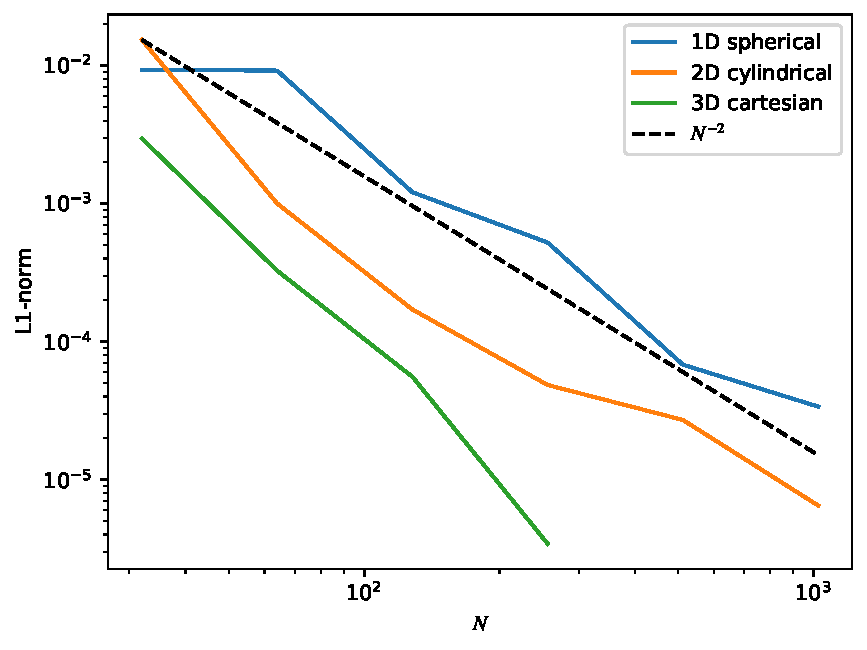
\includegraphics[width=\linewidth]{L1_norm_2.pdf}
  %\caption{A subfigure}
  \label{fig:mg_conv_4}
\end{subfigure}%
\begin{subfigure}{.5\textwidth}
  \centering
  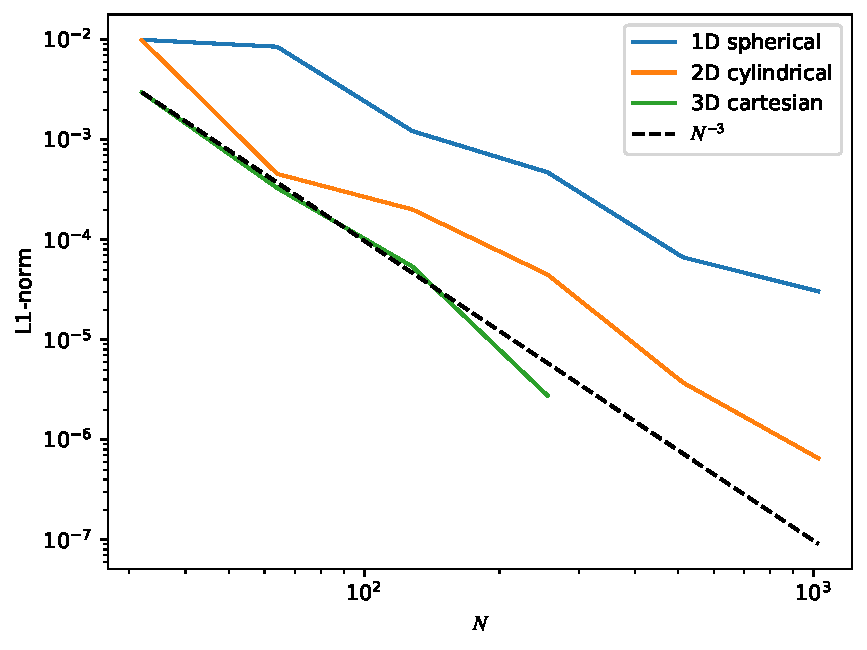
\includegraphics[width=\linewidth]{L1_norm_4.pdf}
  %\caption{A subfigure}
  \label{fig:mg_conv_4}
\end{subfigure}
\caption{L1-norm of $\Phi$ using 2nd order (left) and 4th order central finite difference scheme (right).}
\label{fig:mg_conv}
\end{figure}
Figure \ref{fig:mg_conv} shows the convergent rate of the L1-norm of $\Phi$
\begin{align}
    \left{||} \Phi \right{||}_1 &= \frac{1}{N}\sum^{N}_{i=1} \left| \Phi_i - \Phi^{exact}_i \right|,
\end{align}
where arround second-order accuracy and third-order convergence is achieved for 2nd order and 4th order central finite difference scheme in general.

%********************************** %Second Section  *************************************
\section{Teukolsky wave test}
\label{section4.2}
We consider the quadrupole $(l,m)=(2,0)$ mode of the vacuum solution.
For even-parity quadrupole mode, the metric takes form \cite{teukolsky1982linearized} in spherical coordinate $(r, \theta, \phi)$
\begin{align}
    \begin{split}
    ds^2 =& - dt^2 + \left(1 + A f_{rr}\right) dr^2 + \left(2 B f_{r\theta}\right) r dr d\theta
    + \left(2 B f_{r\phi} \right) r \sin\theta dr d\phi \\
    & \left(1 + C f^{(1)}_{\theta\theta} + A f^{(2)}_{\theta\theta} \right) r^2 d\theta^2
    + \left[2 \left(A-2C\right) f_{\theta\phi} \right] r^2 \sin\theta d\theta d\phi \\
    & + \left(1 + C f^{(1)}_{\phi\phi} + A f^{(2)}_{\phi\phi} \right) r^2 \sin^2\theta d\phi^2,
    \end{split}
\end{align}
where the coefficient $A,B,C$ are constructed from $F(x)$ for $x=t-r$ outgoing wave and $x=t+r$ ingoing wave
\begin{align}
    F(x) = F_1 (t-r) + F_2 (t+r),
\end{align}
and we define
\begin{align}
    F^{(n)} \coloneqq \left. \frac{d^n F_1(x)}{dx^n} \right|_{x=t-r} + (-1)^n \left. \frac{d^n F_2(x)}{dx^n} \right|_{x=t+r}.
\end{align}
Thus, the coefficient are given by
\begin{align}
    A &= 3 \left( \frac{F^{(2)}}{r^3} + \frac{3 F^{(1)}}{r^4} + \frac{3 F}{r^5} \right), \\
    B &= - \left( \frac{F^{(3)}}{r^2} + \frac{3F^{(2)}}{r^3} + \frac{3F^{(1)}}{r^4} + \frac{6F}{r^5} \right), \\
    C &= \frac{1}{4} \left( \frac{F^{(4)}}{r} + \frac{2F^{(3)}}{r^2} + \frac{9F^{(2)}}{r^3} + \frac{21F^{(1)}}{r^4} + \frac{21F}{r^5} \right).
\end{align}
For $m=0$ mode, the angular function $f_{ij}$ are given by
\begin{align}
    f_{rr} &= 2 - 3 \sin^2 \theta, & f_{r\theta} &= - 3 \sin\theta \cos\theta, & f_{r\phi} &= 0, \\
    f_{\theta\theta}^{(1)} &= 3 \sin^2\theta, & f_{\theta\theta}^{(2)} &= -1, & f_{\theta\phi} &= 0, \\
    f_{\phi\phi}^{(1)} &= - f_{\theta\theta}^{(1)}, & f_{\phi\phi}^{(2)} &= 3 \sin^2 \theta - 1.
\end{align}
In our test, we consider 
\begin{align}
    F_1 (x) = - F_2 (x) = \frac{\mathcal{A}}{2} x e^{-\frac{x^2}{\lambda^2}},
\end{align}
and perform the simulation in 2D axisymmetric cylindrical coordinate $(r,z,\phi)$ with $z$ reflection symmetry.
The computational domain covers the region $0\leq \rho \leq 5$, $0\leq z \leq 5$
and the discretization of the domain is set to be $[256,256]$.
The inital profile is given by
\begin{align}\label{eq:Teukolsky_wave_IC}
    \psi &= \alpha = 1, \\
    \beta^i &= 0, \\
    h^{rr} &= \mathcal{A}' \frac{\lambda^4 - \rho^2 z^2}{\lambda^8} e^{-\frac{x^2}{\lambda^2}}, \\
    h^{r z} &= \mathcal{A}' \frac{\rho z \left(\rho^2 - 2 \lambda^2 \right)}{\lambda^8} e^{-\frac{x^2}{\lambda^2}}, \\
    h^{r \phi} &= 0, \\
    h^{zz} &= - \mathcal{A}' \frac{\left(2 \lambda^4 - 4 \lambda^2 \rho^2 + \rho^4 \right)}{\lambda^8} e^{-\frac{x^2}{\lambda^2}}, \\
    h^{z\phi} &= 0, \\
    h^{\phi\phi} &= \mathcal{A}' \frac{\left(\lambda^4 - 4 \lambda^2 \rho^2 +\rho^2 z^2 + \rho^4 \right)}{\lambda^8} e^{-\frac{x^2}{\lambda^2}}, \\
    \hat{A}^{ij} &= 0,
\end{align}
where $\mathcal{A}' = \frac{\mathcal{A}}{12}$.
The analytic solution is written in the Appendix \ref{A3}.
The simulation will be performed under two configurations:
\begin{enumerate}
    %\item Solve the linearized hyperbolic equations only
    %\begin{align}
    %    \partial_t h^{ij} &= 2 \hat{A}^{ij}, \\
    %    \partial_t \hat{A}^{ij} &= \frac{1}{2} f^{kl} \mathcal{D}_k \mathcal{D}_l h^{ij}.
    %\end{align}
    \item Solve the hyperbolic equations only (without elliptic divergence cleaning).
    \label{TW_config_1}
    \item Solve the hyperbolic equations togather with the elliptic sector in FCF except $\psi$, $\alpha$ and $\beta$ (with elliptic divergence cleaning).
    \label{TW_config_2}
\end{enumerate}
In the tests, we choose $\mathcal{A}'=10^{-4}$ and $\lambda=1$.
\begin{figure}[h!]
\centering
  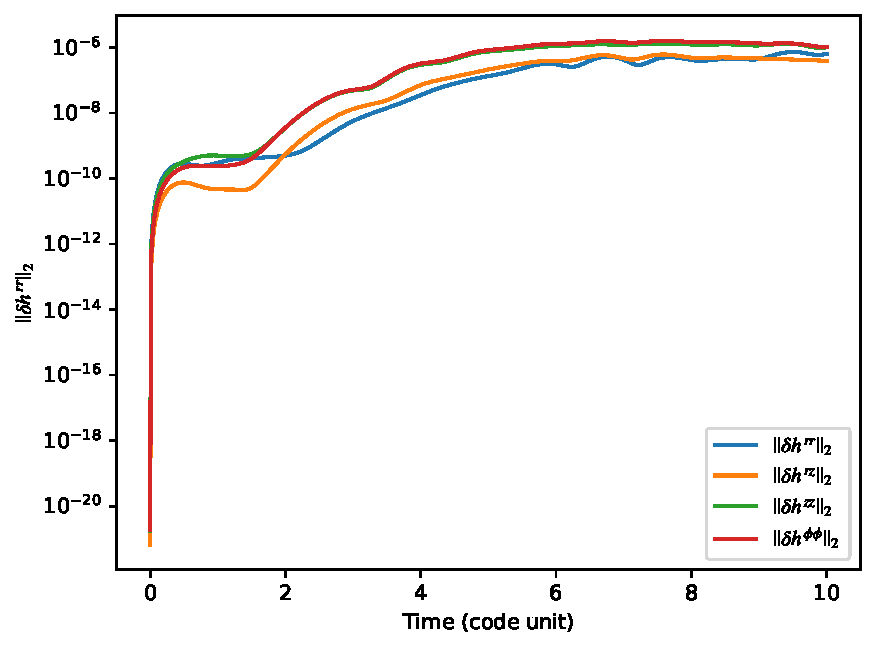
\includegraphics[width=\linewidth]{herr.pdf}
\caption{L2-norm of $h^{ij}$ of the Teukolsky wave test by solving hyperbolic equations without elliptic sector (configuration \ref{TW_config_1}).}
\label{fig:TW_h_err}
\end{figure}
In figure \ref{fig:TW_h_err},
it shows the L2-norm of $h^{ij}$ which is given by
\begin{align}
    \delta h^{ij} &= \sqrt{\frac{1}{V}\sum \left| h^{ij} - h^{ij}_{exact} \right|^2}.
\end{align}
The simulation result agrees with the analytical solution very well.
\begin{figure}[h!]
\centering
\begin{subfigure}{.5\textwidth}
  \centering
  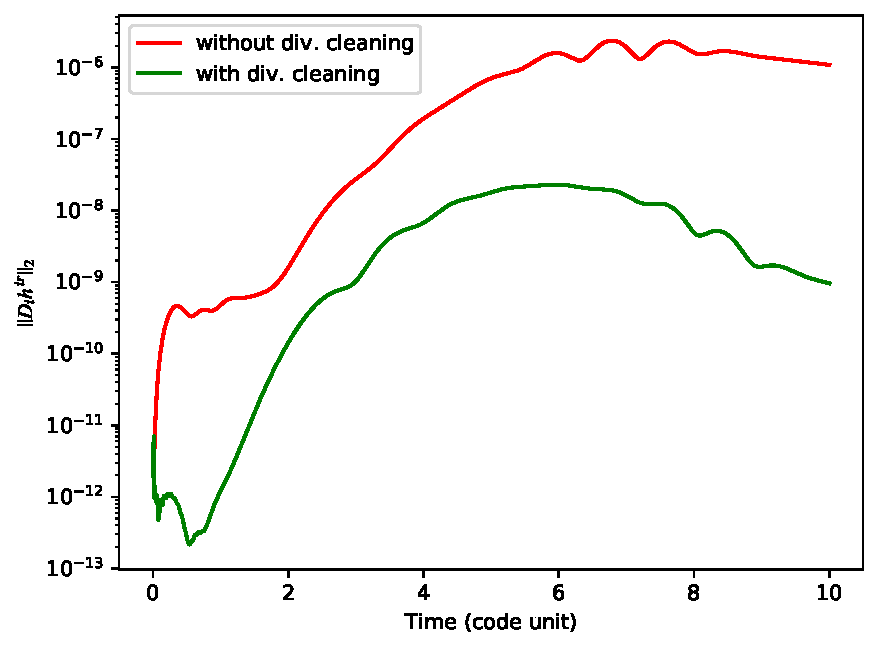
\includegraphics[width=\linewidth]{Dh1.pdf}
  \caption{L2-norm of $\mathcal{D}_i h^{ir}$}
  \label{fig:Dh1}
\end{subfigure}%
\begin{subfigure}{.5\textwidth}
  \centering
  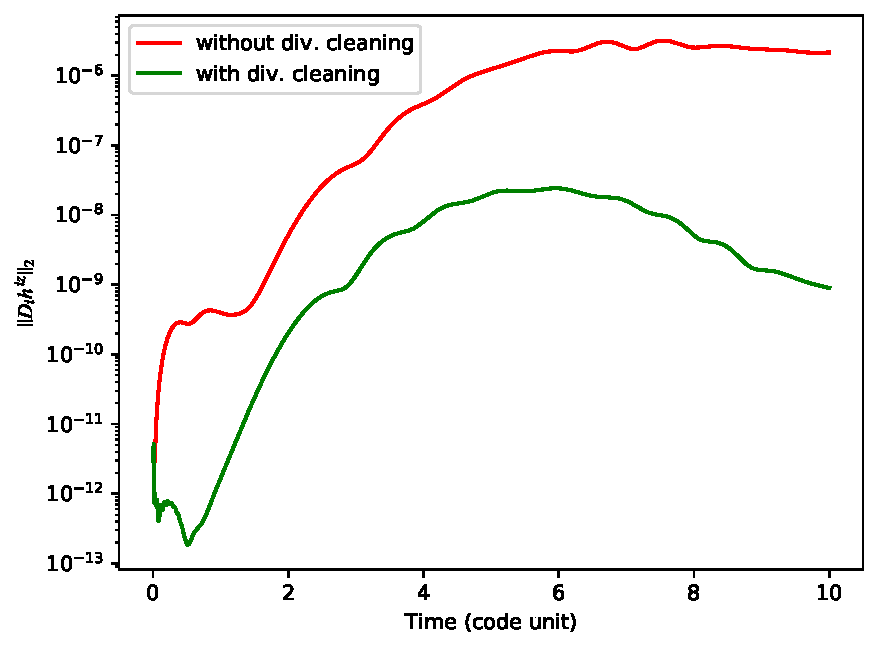
\includegraphics[width=\linewidth]{Dh2.pdf}
  \caption{L2-norm of $\mathcal{D}_i h^{iz}$}
  \label{fig:Dh2}
\end{subfigure}
\caption{L2-norm of the divergence of $h^{ij}$.
The red line corresponds to the evolution of $h^{ij}$ without divergence cleaning
while the green line corresponds to the evolution of $h^{ij}$ with divergence cleaning.}
\label{fig:Dh}
\end{figure}
In figure \ref{fig:Dh}, it shows that the elliptic divergence cleaning method is effective on
reducing the divergence of $h^{ij}$.
Especially for $t \gtrsim 5$ when the wave is propagated out of the computational domain,
the divergence of $h^{ij}$ keep increasing if no treatment is applied,
while it is suppressed with the elliptic cleaning method.
\begin{figure}[h!]
\centering
\begin{subfigure}{.5\textwidth}
  \centering
  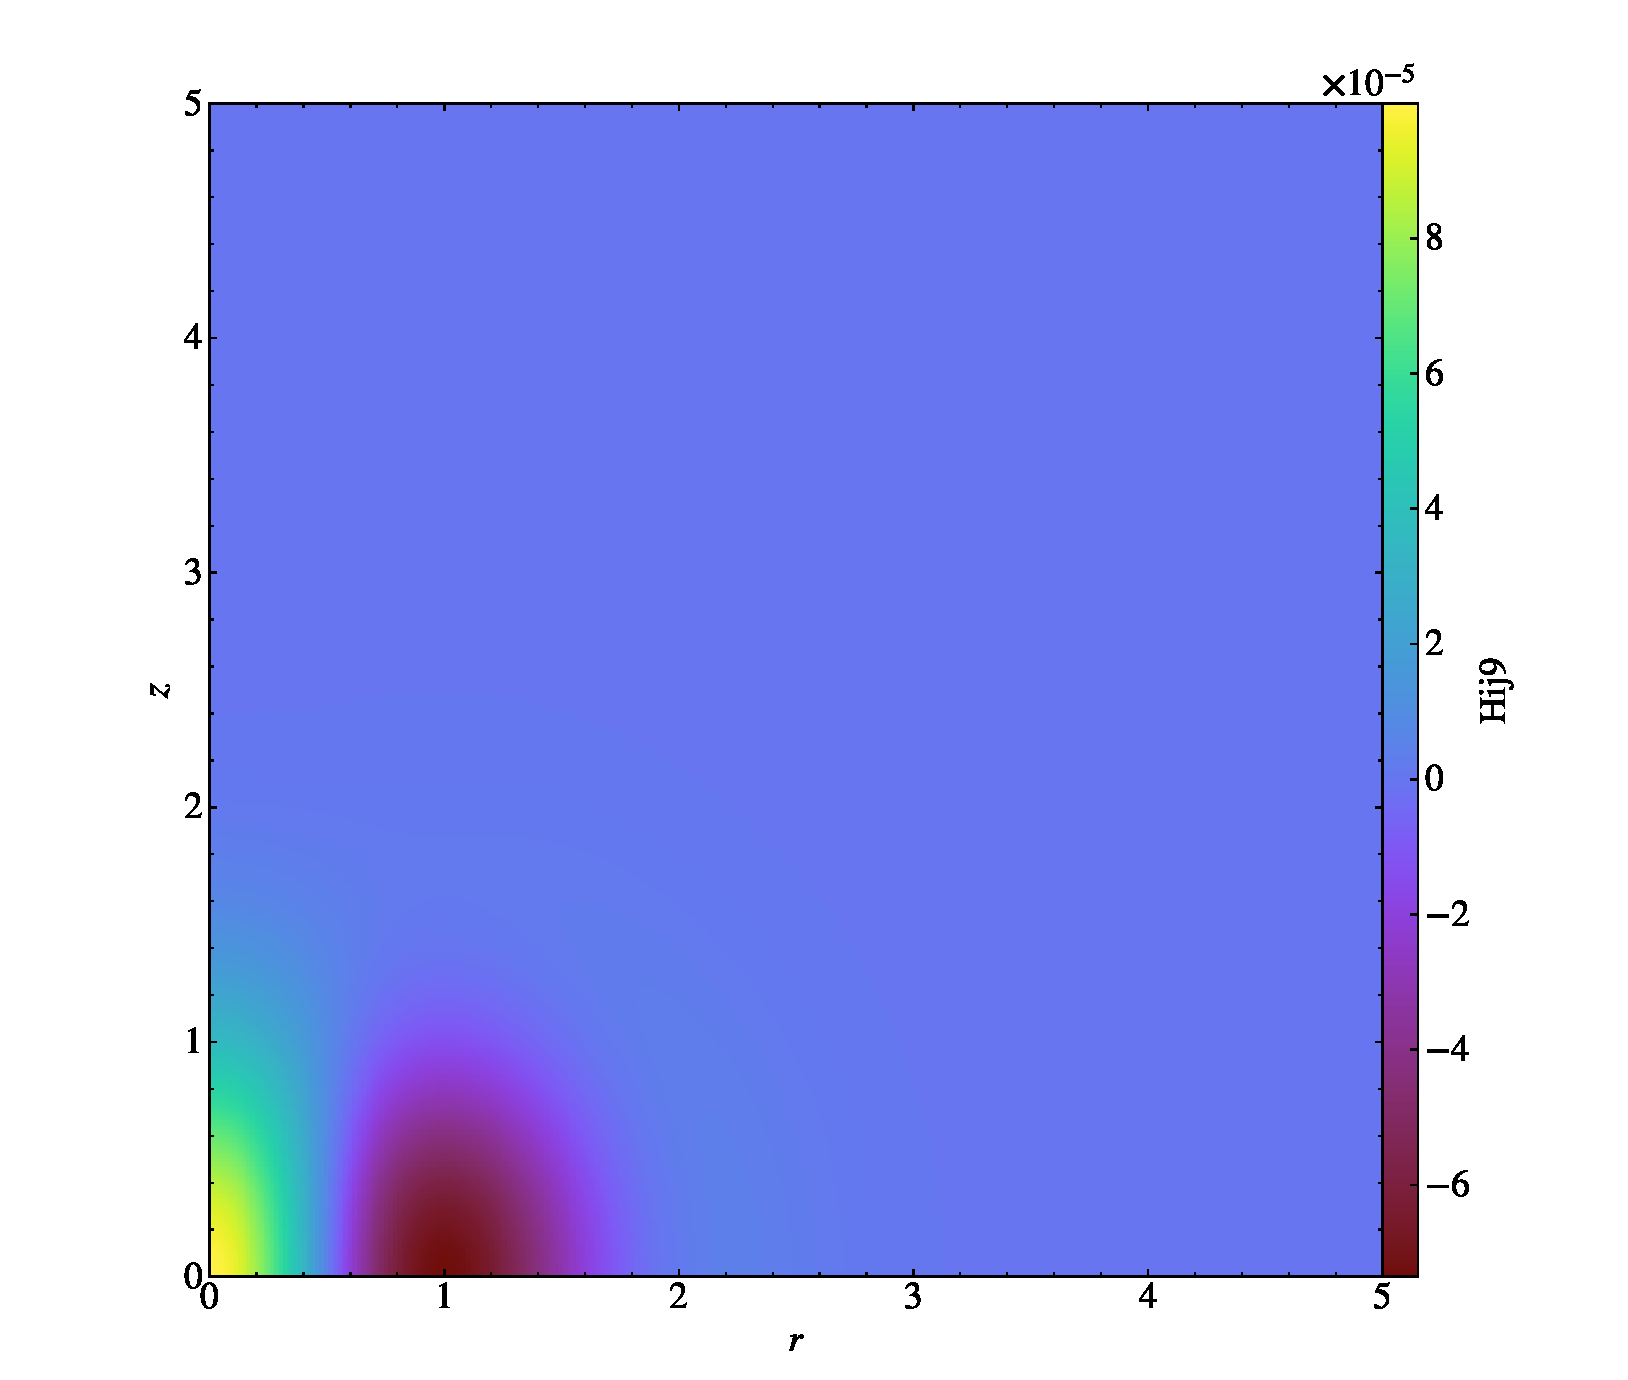
\includegraphics[width=\linewidth]{result_hij_0000.pdf}
  %\caption{L2-norm of $\mathcal{D}_i h^{ir}$}
  \label{fig:hij9_0}
\end{subfigure}%
\begin{subfigure}{.5\textwidth}
  \centering
  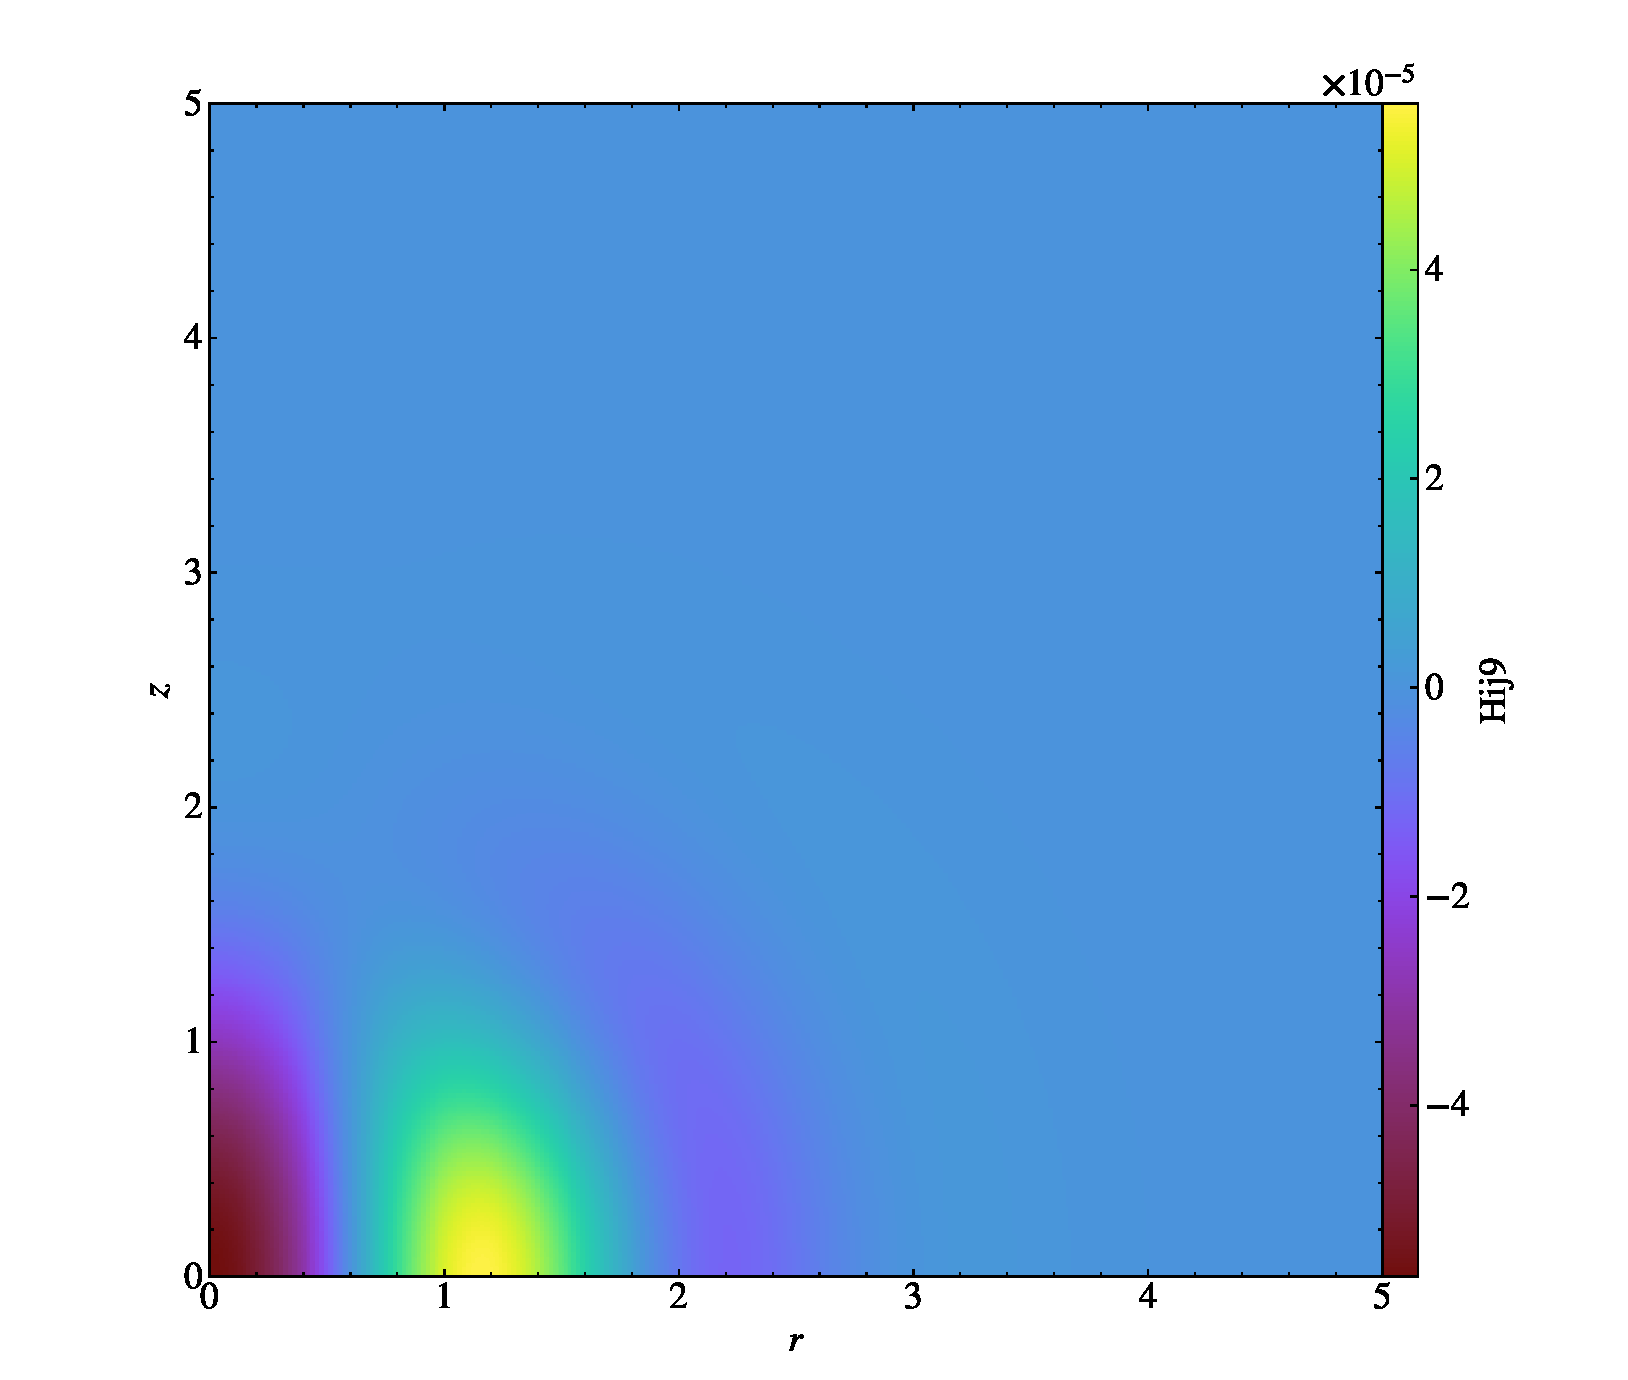
\includegraphics[width=\linewidth]{result_hij_0010.pdf}
  %\caption{L2-norm of $\mathcal{D}_i h^{ir}$}
  \label{fig:hij9_1}
\end{subfigure}%

\begin{subfigure}{.5\textwidth}
  \centering
  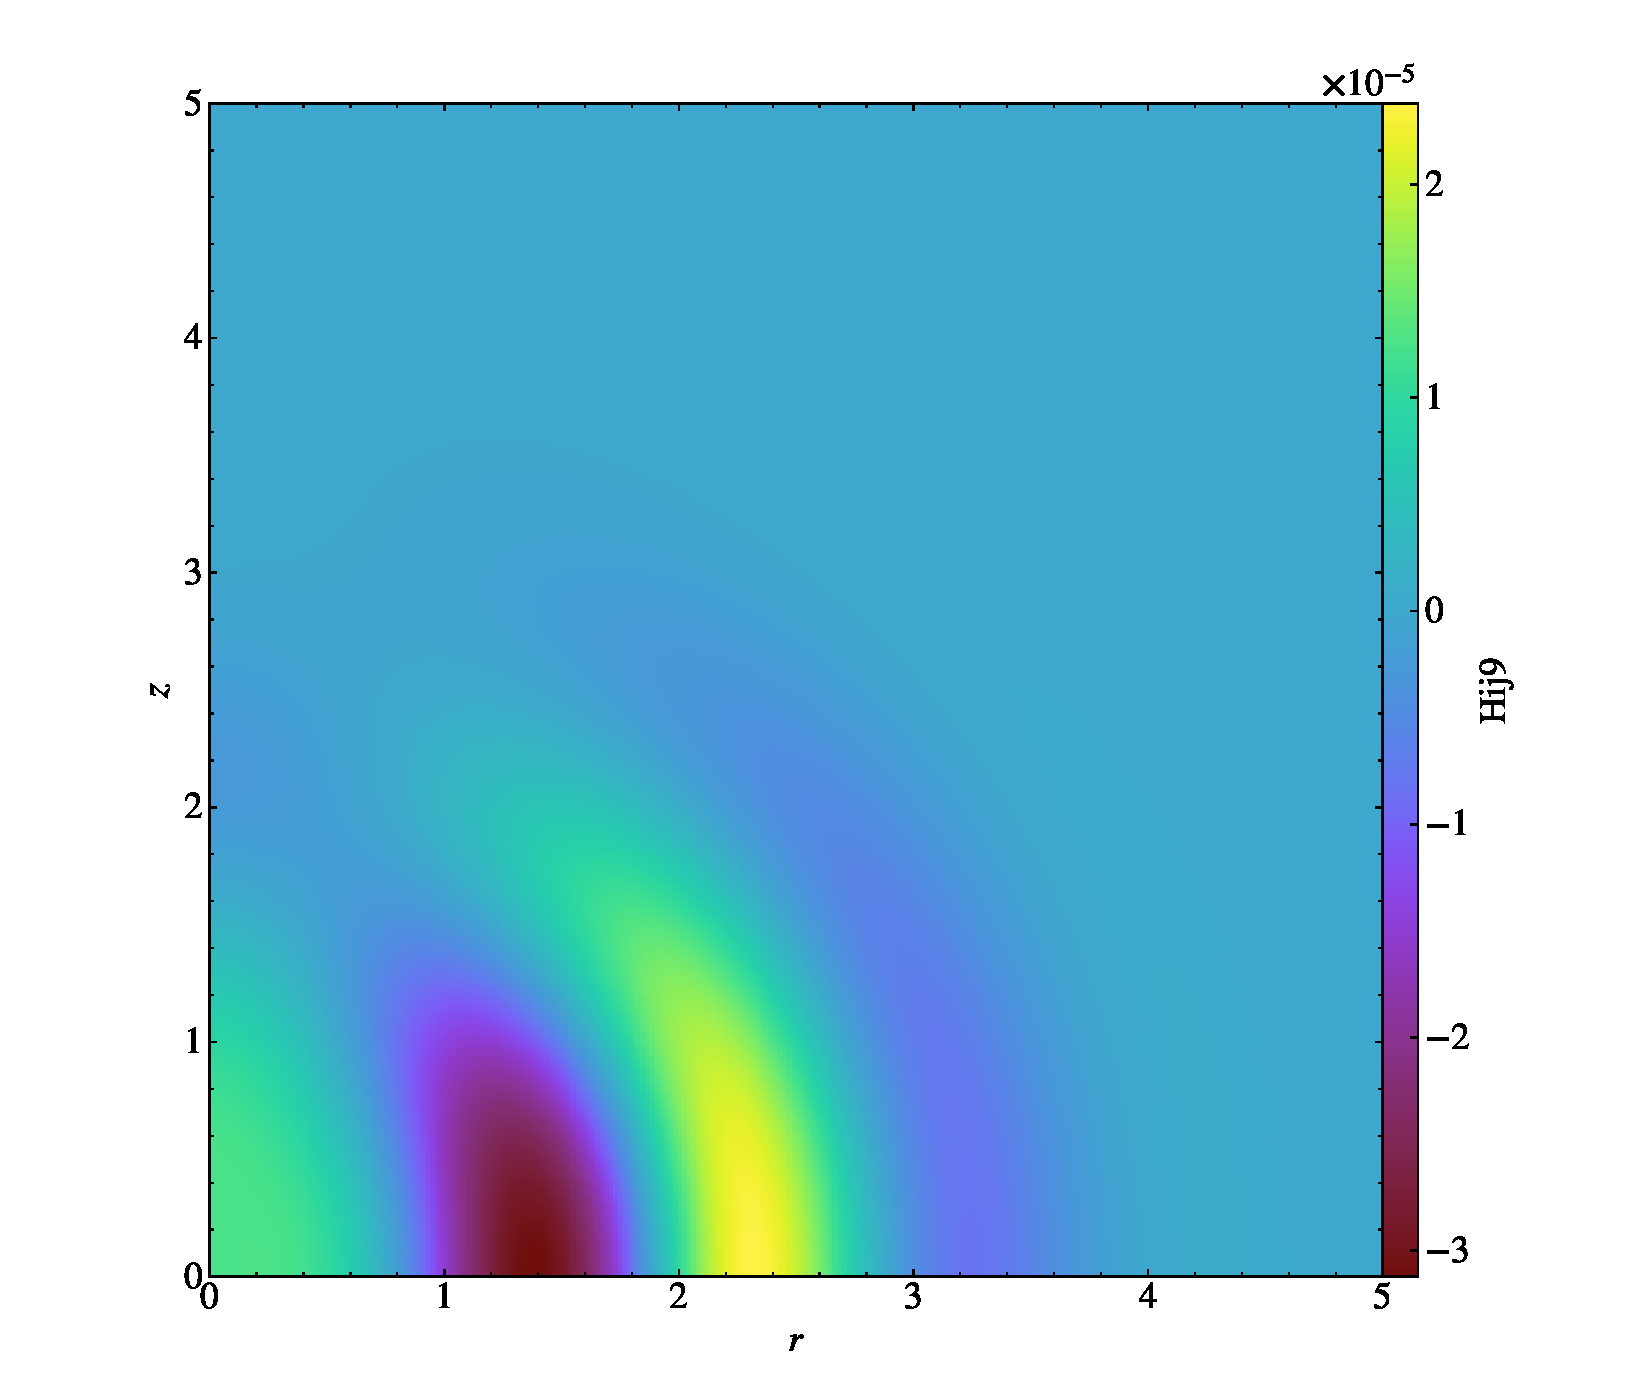
\includegraphics[width=\linewidth]{result_hij_0020.pdf}
  %\caption{L2-norm of $\mathcal{D}_i h^{ir}$}
  \label{fig:hij9_2}
\end{subfigure}%
\begin{subfigure}{.5\textwidth}
  \centering
  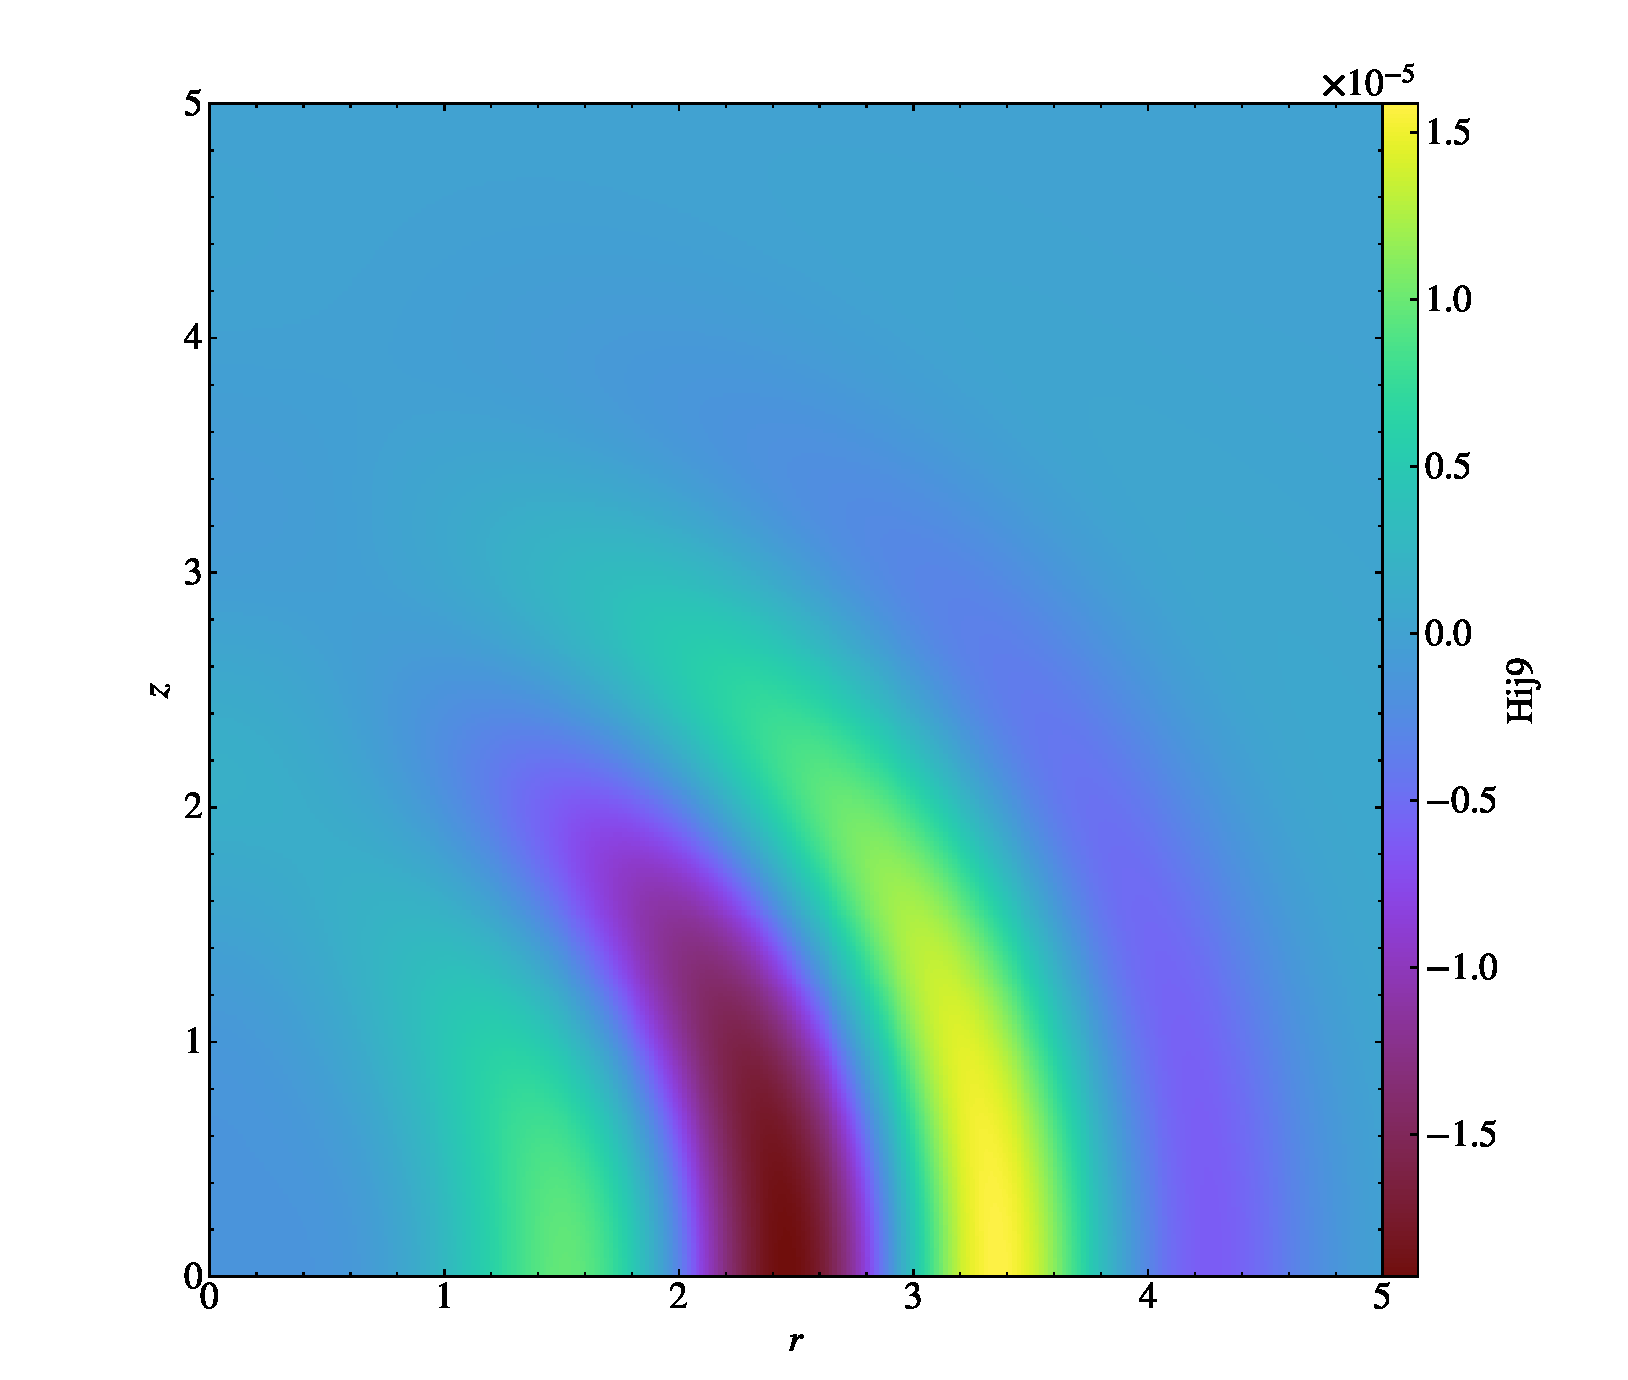
\includegraphics[width=\linewidth]{result_hij_0030.pdf}
  %\caption{L2-norm of $\mathcal{D}_i h^{ir}$}
  \label{fig:hij9_3}
\end{subfigure}%

\begin{subfigure}{.5\textwidth}
  \centering
  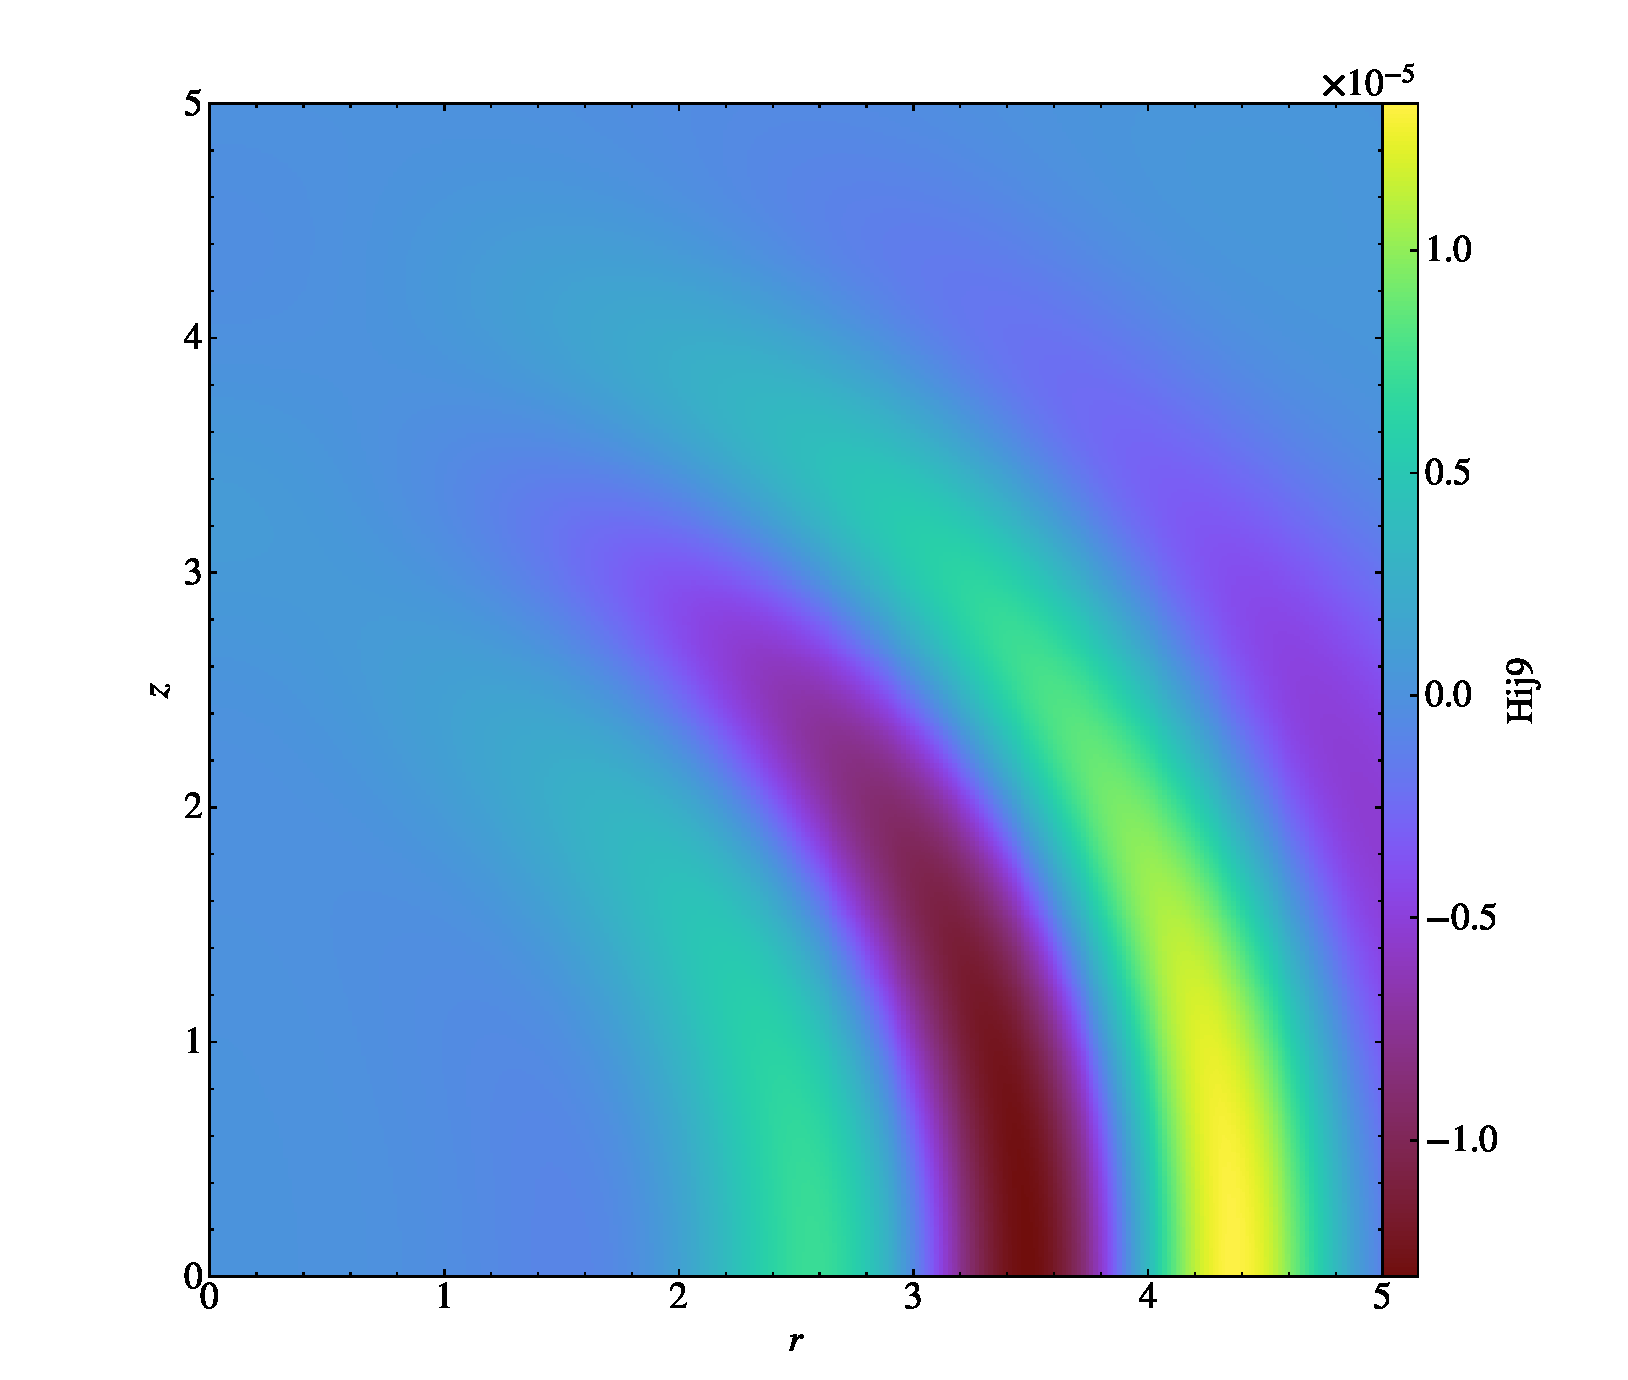
\includegraphics[width=\linewidth]{result_hij_0040.pdf}
  %\caption{L2-norm of $\mathcal{D}_i h^{ir}$}
  \label{fig:hij9_4}
\end{subfigure}%
\begin{subfigure}{.5\textwidth}
  \centering
  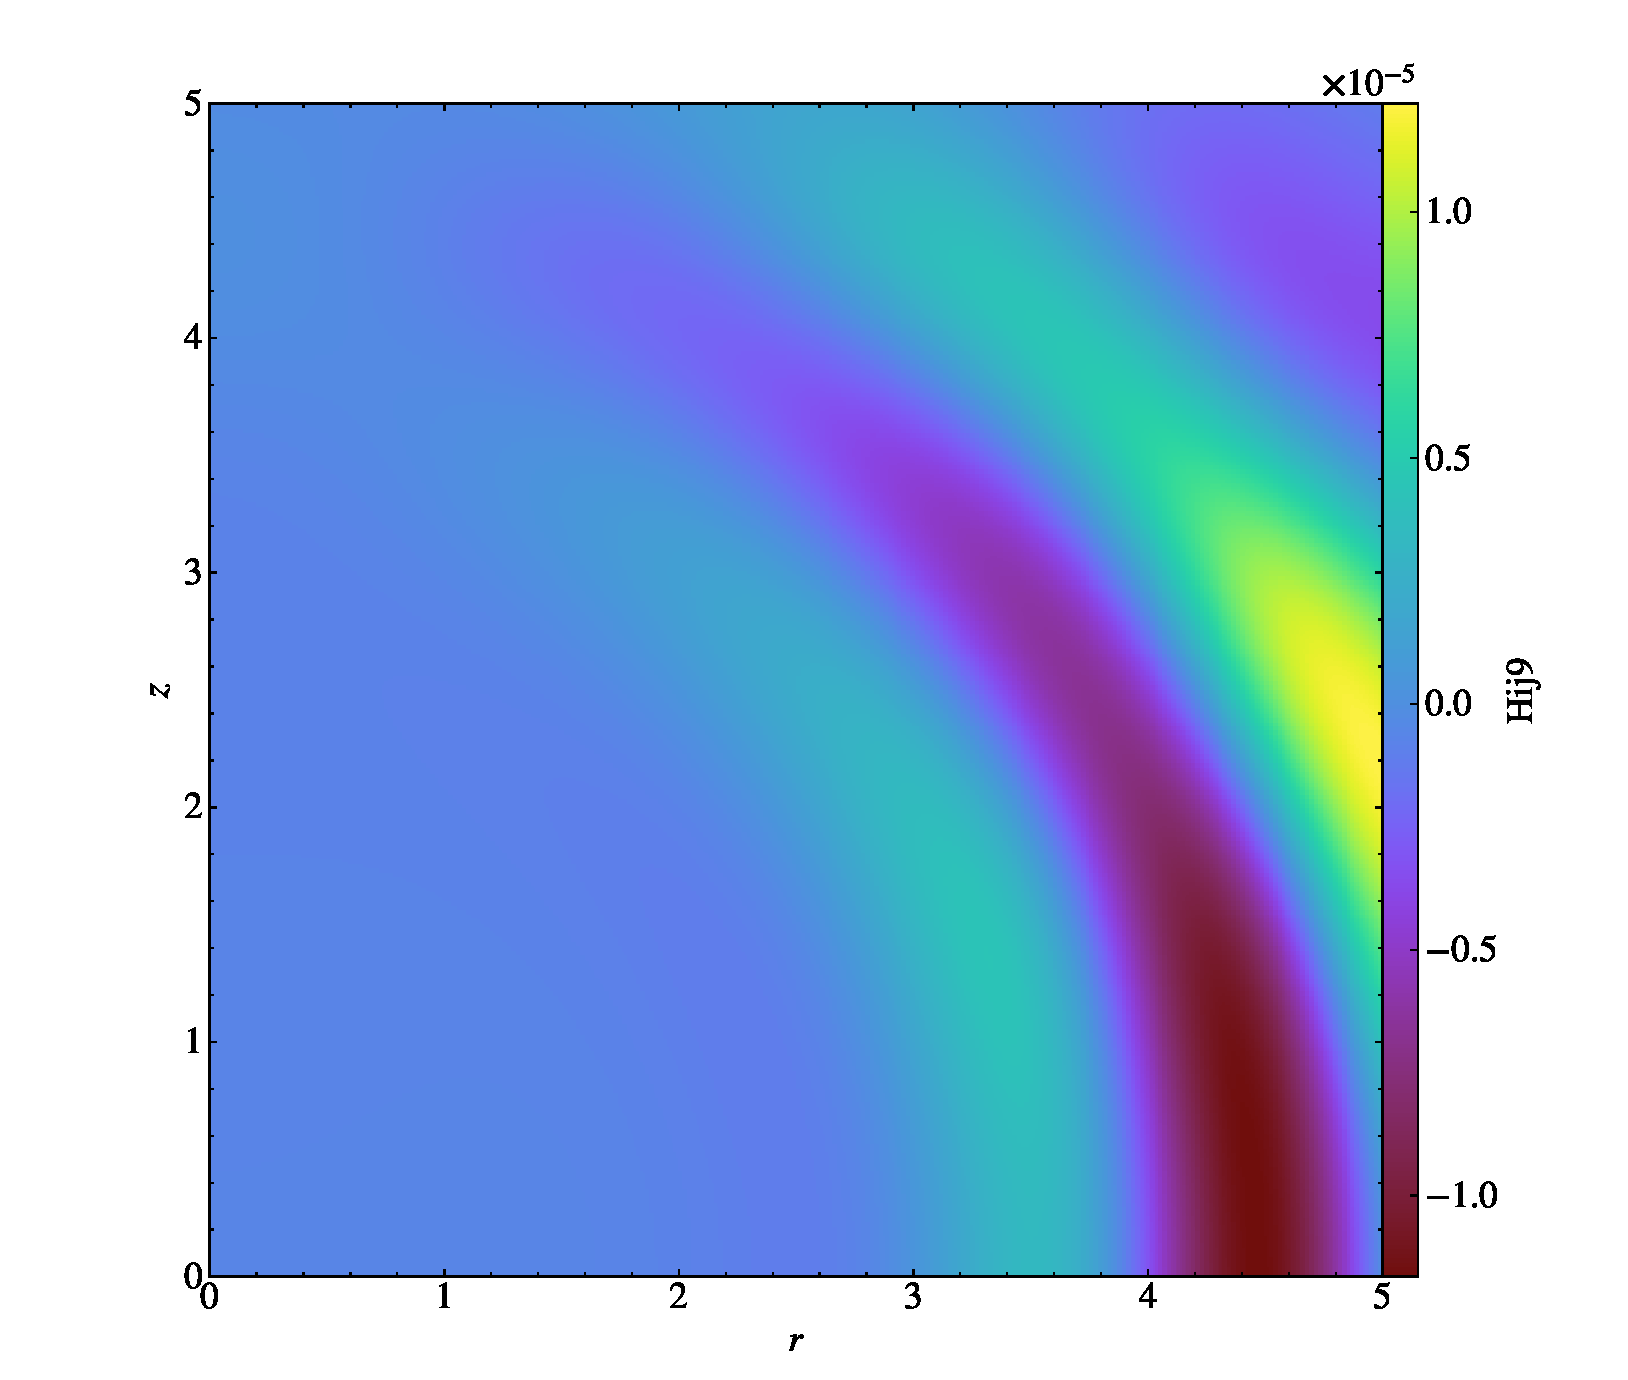
\includegraphics[width=\linewidth]{result_hij_0050.pdf}
  %\caption{L2-norm of $\mathcal{D}_i h^{ir}$}
  \label{fig:hij9_5}
\end{subfigure}%

\caption{Evolution of $h^{\phi\phi}$ component between $t=0$ (upper left) and $t=5$ (lower right) with elliptic divergence cleaning.}
\label{fig:hij9}
\end{figure}
In figure \ref{fig:hij9}, we show the evolution of the $h^{\phi\phi}$ component with elliptic divergence cleaning.

%********************************** %Third Section  *************************************
\section{General relativistic hydrodynamics in dynamic spacetime} %Section - 4.3
\label{section4.3}
Here we study the evolution of a neutron star with dynamical background under FCF scheme and passive FCF scheme.
\subsection{Non-rotating neutron star}
\label{section4.3.1}
In this test, we consider a non-rotating neutron star known as "BU0" \cite{dimmelmeier2006non}
which is constructed with the polytropic index $\Gamma = 2$ and $K = 100$,
and central rest-mass density $\rho_c = 1.28 \times 10^{-3}$ (in $c=G=M_\odot=1$ unit).
This star model is generated by the open-source code \texttt{XNS} 
\cite{bucciantini2011general,pili2014axisymmetric,pili2015general,pili2017general}.
We simulate the star in 2D cylindrical coordinate and impose $z$ reflection symmetry.
The computational domain covers $0 \leq r \leq 60$, $0\leq z \leq 60$ in code unit
with resolution $n_r \times n_z = 256 \times 256$.
The ideal-gas equation of state with $\Gamma = 2$ is used for the simulation.
We extract the plus polarization of gravitational wave signal $h_{+}$ at $(r_{ext}, z_{ext}) = (40, 0)$ which is given by
\begin{align}
    h_{+} \approx \frac{h^{\phi\phi} - h^{zz}}{2} \frac{R_{ext}}{R},
\end{align}
where $R=\sqrt{r^2+z^2}$ is the extraction radius.\\
\begin{figure}[h!]
\centering
  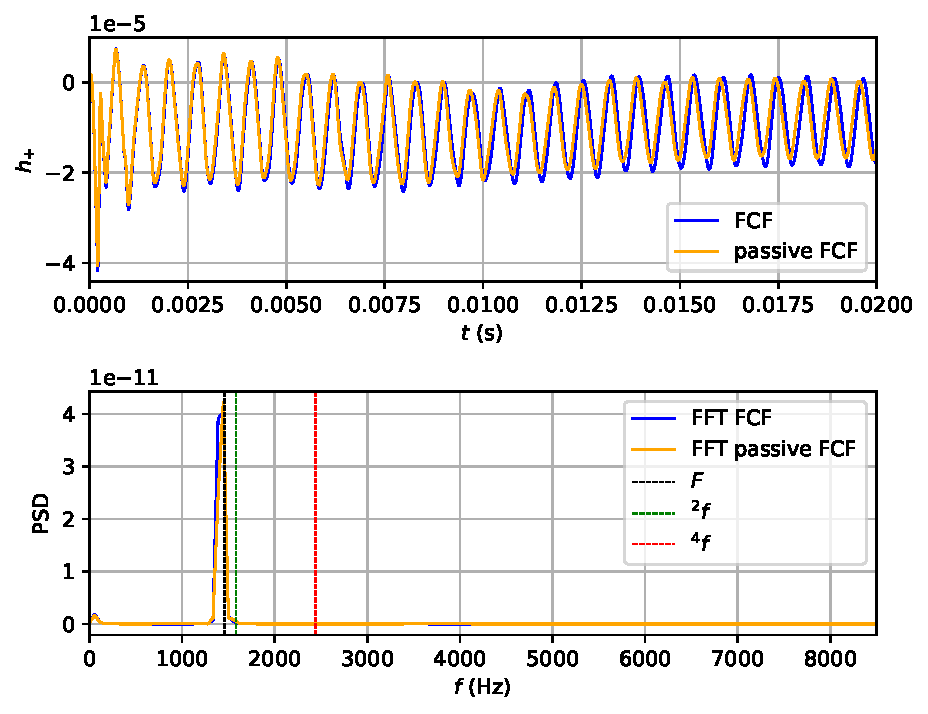
\includegraphics[width=\linewidth]{GW_combine_h_BU0.pdf}
\caption{(upper panel) $h_{+}$ extracted at $(r_{ext}, z_{ext}) = (40, 0)$ from the simulations of oscillating neutron star "BU0".
(lower panel) The power spectral density of $h_{+}$.
The vertical lines represent the known and well-tested eigenmode frequencies \cite{dimmelmeier2006non}}
\label{fig:GW_h_BU0}
\end{figure}
Figure \ref{fig:GW_h_BU0} shows the extracted gravitational wave signal $h_{+}$ from "BU0".
Note that since the BU0 is a shperically symmetric star and it is simulated without any initial perturbation,
only $F$ mode can be extracted which its value agrees with \cite{dimmelmeier2006non}.

\subsection{Rapidly rotating neutron star}
\label{section4.3.2}
In this test, we consider a rapidly-rotating neutron star known as "BU8" \cite{dimmelmeier2006non}.
The polytropic index, $K$ value and central rest-mass density are the same as "BU0",
except that it is uniformly rotating at an angular velocity of $\Omega = 2.633 \times 10^{-2}$.
The simulation setups are same as section \ref{section4.3.1},
and again we extracted $h_{+}$ at $(r_{ext}, z_{ext}) = (40, 0)$.\\
\begin{figure}[h!]
\centering
  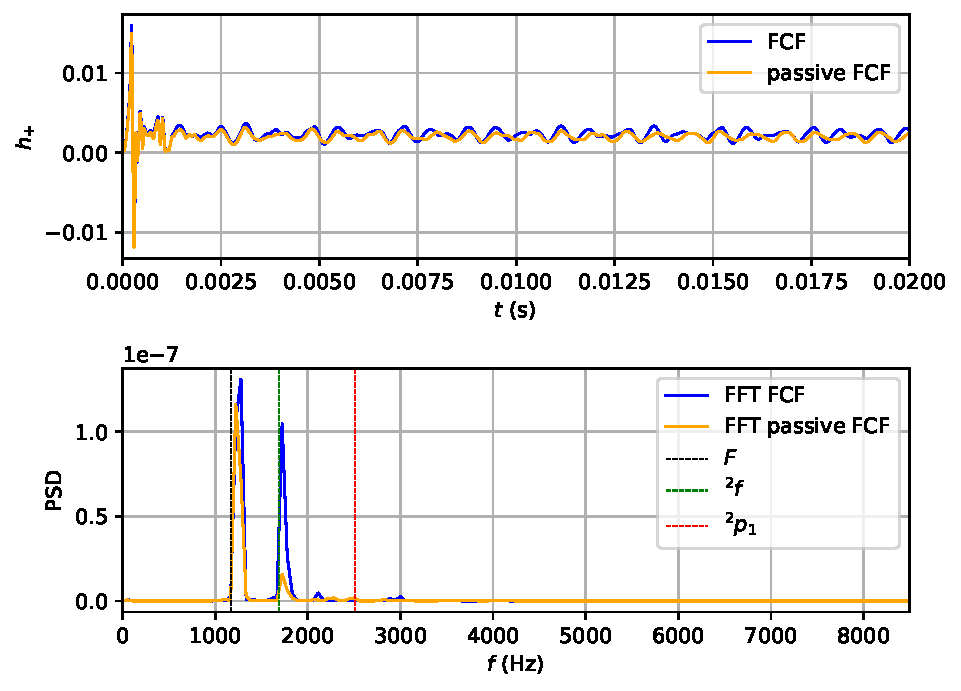
\includegraphics[width=\linewidth]{GW_combine_h_BU8.pdf}
\caption{(upper panel) $h_{+}$ extracted at $(r_{ext}, z_{ext}) = (40, 0)$ from the simulations of oscillating neutron star "BU8".
(lower panel) The power spectral density of $h_{+}$ calculated from $t=2.5ms$ due to the spurios oscillation at the beginning.
The vertical lines represent the known and well-tested eigenmode frequencies \cite{dimmelmeier2006non}}
\label{fig:GW_h_BU8}
\end{figure}
Figure \ref{fig:GW_h_BU8} shows the extracted gravitational wave signal $h_{+}$ from "BU8".
The extracted pulsation mode agrees with \cite{dimmelmeier2006non} for $F$ and ${}^2f$ mode.
Note that the initial profile "BU8" is constructed under CFC approximation with zero $h^{ij}$,
which is not the case when full GR is considered.
This is why a spurious oscillation in $h$ occurs at the beginning of the simulation.
Nonetheless, $h$ quickly settles down and oscillates around the new equilibrium position.
We also observed that the ${}^2f$ mode of $h_+$ in FCF scheme has a higher amplitude compared to passive FCF scheme.



% ******************************* Part III *************************************
\part{Conclusion}\label{part3}
%!TEX root = ../thesis.tex
%*******************************************************************************
%*********************************** Fifth Chapter *****************************
%*******************************************************************************

\chapter{Concluding Remarks}  %Title of the Fifth Chapter

\ifpdf
    \graphicspath{{Chapter5/Figs/PDF/}{Chapter5/Figs/}}
\else
    \graphicspath{{Chapter5/Figs/}}
\fi
The main theme of this work is to extend the \texttt{Gmunu} code to adopt the
fully constrained formulation (FCF) scheme,
a full general relativistic formulation naturally generalized from the conformally flat condition (CFC) approximation
which is current used in the code.
So far only two dimensional cylindrical coordinate is implemented for the FCF scheme.
In this thesis, we present the methodology and implementation of \texttt{Gmunu} in detail.\\
We have tested \texttt{Gmunu} with several benchmarking tests.
In the Teukolsky wave test, we have shown the stability and convergence of evolving the hyperbolic equations in FCF.
We also demonstrated that the elliptic divergence cleaning using multigrid method is able to maintain the gauge condition.
For the hydrodynamics,
we have performed simulations of the evolution of both non-rotating and rotating neutron stars.
We are able to extract the gravitational wave signature directly from the metric components.

%********************************** %First Section  **************************************
\section*{Future Plan}
Here, we list some possible improvement of \texttt{Gmunu} planned for the future.

\paragraph{Support different geometries}
Currently, the FCF scheme is only implemented in 2D cylindrical coordinate
which limit our study to axisymmetric profiles.
We will extend the code to support 2D spherical
as well as 3D spherical/Cartesian coordinates in the future
so that we can broaden our study to non-axisymmetric systems
such as binary systems and supernovae.

\paragraph{Simulate black holes}
In \texttt{Gmunu}, we have no treatment to handle the black holes singularity nor the apparent horizon.
It has been shown that the excision scheme can be used to deal with black holes for constrained evolution scheme in spherically symmetric spacetime \cite{cordero2014excision}.
Therefore, we would like to develop a horizon finder in \texttt{Gmunu} and implement the excision scheme in the future.

\paragraph{Improve the FCF scheme}
We used finite difference for solving Einstein equations and finite volume for solving the hydrodynamics.
Although they are equivalent in the case of second order accuracy,
this becomes a problem if we extend the code to high-order numerical methods in the future.
It has been suggested that the hyperbolic sector in FCF can be rewritten in conservative form \cite{cordero2008mathematical}.
Therefore, we would like to rewrite the hyperbolic equations in FCF to suit the finite volume scheme in the future.

%\include{Chapter6/chapter6}
%\include{Chapter7/chapter7}



% ********************************** Back Matter *******************************
% Backmatter should be commented out, if you are using appendices after References
%\backmatter

% ********************************** Bibliography ******************************
\begin{spacing}{0.9}

% To use the conventional natbib style referencing
% Bibliography style previews: http://nodonn.tipido.net/bibstyle.php
% Reference styles: http://sites.stat.psu.edu/~surajit/present/bib.htm

\bibliographystyle{aasjournal}
%\bibliographystyle{apalike}
%\bibliographystyle{unsrt} % Use for unsorted references  
%\bibliographystyle{plainnat} % use this to have URLs listed in References
\cleardoublepage
%\bibliography{References/references} % Path to your References.bib file


% If you would like to use BibLaTeX for your references, pass `custombib' as
% an option in the document class. The location of 'reference.bib' should be
% specified in the preamble.tex file in the custombib section.
% Comment out the lines related to natbib above and uncomment the following line.

\printbibliography[heading=bibintoc, title={References}]


\end{spacing}

% ********************************** Appendices ********************************

\begin{appendices} % Using appendices environment for more functunality

%!TEX root = ../thesis.tex
% ******************************* Thesis Appendix A ****************************
\chapter{Useful relations for implementation of constrained scheme}

\section{The elliptic equations in constrained scheme}
\section{Generalized Dirac gauge conditions}

%!TEX root = ../thesis.tex
% ******************************* Thesis Appendix B ********************************

\chapter{Reference flat metric in 3D}



\end{appendices}

% *************************************** Index ********************************
\printthesisindex % If index is present

\end{CJK}
\end{document}
